\documentclass[sigconf,review,anonymous]{acmart}

\AtBeginDocument{%
  \providecommand\BibTeX{{%
    Bib\TeX}}}

% RecSys 2026 submission mode (anonymous review).
% For camera-ready, switch documentclass to [sigconf] and replace rights metadata
% below with the exact values from ACM rights management.
\setcopyright{none}
\acmConference[RecSys '26]{Proceedings of the 20th ACM Conference on Recommender Systems}{September 28--October 2, 2026}{Minneapolis, MN, USA}
\acmBooktitle{Proceedings of the 20th ACM Conference on Recommender Systems (RecSys '26), September 28--October 2, 2026, Minneapolis, MN, USA}
\acmDOI{}
\acmISBN{}

\usepackage{array}
\usepackage{dblfloatfix}
\usepackage{float}
\usepackage{makecell}
\usepackage{multirow}
\usepackage{placeins}
\usepackage{subcaption}
\usepackage{tabularx}
\usepackage[table]{xcolor}

\raggedbottom
\setlength{\emergencystretch}{2em}
\setcounter{topnumber}{3}
\setcounter{dbltopnumber}{2}
\renewcommand{\topfraction}{0.9}
\renewcommand{\dbltopfraction}{0.9}
\renewcommand{\textfraction}{0.07}
\renewcommand{\floatpagefraction}{0.8}
\renewcommand{\dblfloatpagefraction}{0.8}
\setlength{\textfloatsep}{10pt plus 2pt minus 2pt}
\setlength{\dbltextfloatsep}{9pt plus 2pt minus 2pt}
\setlength{\floatsep}{8pt plus 2pt minus 2pt}
\setlength{\dblfloatsep}{8pt plus 2pt minus 2pt}
\setlength{\intextsep}{8pt plus 2pt minus 2pt}

\newcolumntype{Y}{>{\centering\arraybackslash}X}
\newcolumntype{L}[1]{>{\raggedright\arraybackslash}p{#1}}
\definecolor{routerecgray}{RGB}{242,242,242}
\newcommand{\tblbest}[1]{\textbf{#1}}
\newcommand{\tblsecond}[1]{\underline{#1}}
\newcommand{\placeholderpanel}[1]{\fbox{\rule{0pt}{#1}\rule{0.92\linewidth}{0pt}}}
\newcommand{\jm}[1]{{\color{red} #1}}

\begin{document}

\title[RouteRec for Sequential Recommendation]{RouteRec: Behavior-Guided Sparse Routing for Sequential Recommendation}

\author{First Author}
\affiliation{%
  \institution{KAIST}
  \department{Kim Jaechul Graduate School of AI}
  \city{Daejeon}
  \country{Republic of Korea}}
\email{first.author@kaist.ac.kr}

\author{Second Author}
\affiliation{%
  \institution{KAIST}
  \department{Kim Jaechul Graduate School of AI}
  \city{Daejeon}
  \country{Republic of Korea}}
\email{second.author@kaist.ac.kr}

\renewcommand{\shortauthors}{Author et al.}

\begin{abstract}
Session-based recommendation models have explored many ways to make use of behavioral context --- cross-session history, temporal structure, side information --- to better capture what a user is likely to want next. We are interested in a specific direction: using behavioral patterns to differentiate the computation applied to each session, rather than only enriching a shared representation. Mixture of Experts (MoE) makes this possible: a router selects which expert subset processes each input, allowing different sessions to follow different computation paths. The key question is what should drive that routing decision.

Hidden states are shaped by next-item prediction rather than behavioral character. Routing from them ties routing control to the very representation it is meant to influence, making it hard to separate what drives route changes from what drives prediction changes. \textbf{RouteRec} instead computes \emph{behavioral cues} (compact statistics derived directly from interaction logs) on a control path kept separate from the sequential backbone, and uses them to select which experts process each session. Because cues are computed from the raw log rather than from the prediction objective, route choices trace back to specific, observable behavioral quantities. Cues are extracted at three temporal scopes (macro, mid, micro) and fed into a hierarchical sparse router that concentrates computation on a small, focused expert subset.

RouteRec achieves the best overall seen-target ranking across six datasets under a shared sessionized temporal protocol, with the clearest gains on Foursquare, LastFM, and KuaiRec. In the main comparison, it leads with an overall Avg.~Rank of 1.67 versus 3.56 for the next-best baseline. Routing diagnostics confirm that expert selection shifts consistently with observed behavioral patterns. Anonymous code: \url{https://anonymous.4open.science/r/RouteRec/}.
\end{abstract}

\begin{CCSXML}
<ccs2012>
 <concept>
  <concept_id>10002951.10003317.10003347.10003350</concept_id>
  <concept_desc>Information systems~Recommender systems</concept_desc>
  <concept_significance>500</concept_significance>
 </concept>
</ccs2012>
\end{CCSXML}

\ccsdesc[500]{Information systems~Recommender systems}

\keywords{sequential recommendation, sparse routing, conditional computation, behavioral cues, mixture of experts}

\maketitle

\section{Introduction}
\label{sec:intro}

Session-based recommendation predicts the next item from a user's current session~\cite{wang2021sessionsurvey,jannach2022sessions}.
Since a single session often carries limited signals on its own, previous works have looked beyond it, drawing on the user's past sessions~\cite{quadrana2017hrnn}, cross-user patterns~\cite{kang2018sasrec}, and interaction-level side information such as timestamps and categories~\cite{li2020tisasrec,zhang2019fdsa}.
We refer to this broader evidence as \emph{behavioral context}: the cross-session history and interaction-level patterns that a model can exploit beyond the current session.
Recent works have proposed hierarchical cross-session encoders~\cite{quadrana2017hrnn,ying2018shan}, temporal attention biases~\cite{li2020tisasrec}, and side-information fusion~\cite{zhang2019fdsa,xie2022difsr} to leverage this behavioral context.
However, they rely on a shared backbone that processes every session through the same computational path, regardless of how that session actually behaves (Figure~\ref{fig:intro-behavioral-features}).

\begin{figure}[!t]
  \centering
  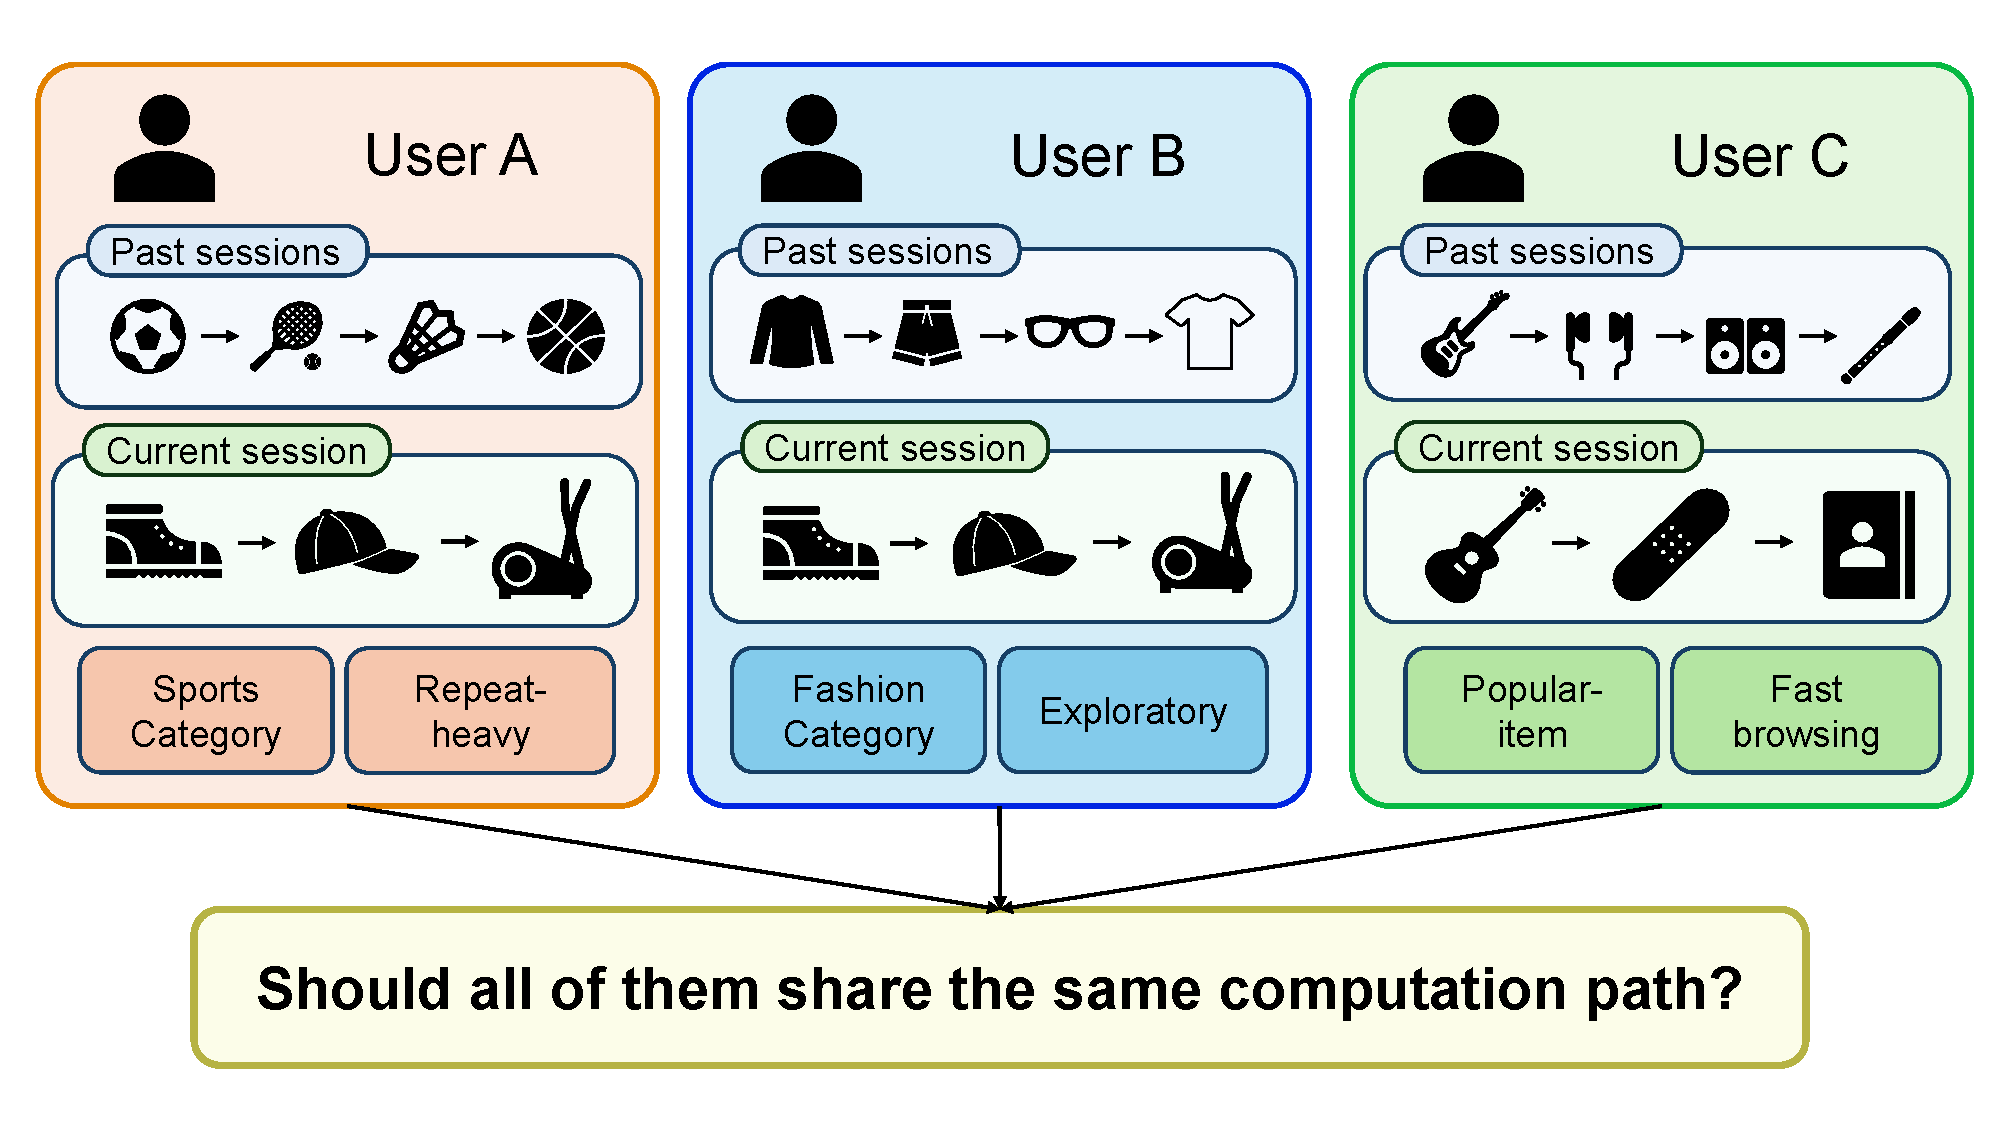
\includegraphics[width=\columnwidth]{figures/figure1_different_user.pdf}
  \caption{In standard sequential recommendation, the same computation path is applied to sessions with distinct behavioral characteristics, regardless of differences in pace, repetition, or category focus.}
  % \Description{A problem-motivation figure contrasting different user and session behavior patterns, showing that behaviorally different cases are processed with the same computation path in standard sequential recommendation.}
  \label{fig:intro-behavioral-features}
\end{figure}

Mixture of experts (MoE)~\cite{jacobs1991adaptive,jordan1994hme} offers a natural mechanism for mitigating this uniformity by replacing a shared transformation with multiple experts selected by a learned router.
In sequential recommender systems, the router is typically conditioned on the hidden states of the backbone model.
Such a design makes routing behavior guided by the learned representations rather than by the behavioral characteristics of the session.

We take the position that behavioral context should determine \emph{which computation path} is applied, not only what a shared block encodes. Moreover, this routing signal should be computed directly from interaction logs rather than read from hidden states. In short sessions, pace, repetition style, and category concentration are directly visible in the raw log before any model transformation. Hidden states optimized for next-item prediction do not explicitly organize these patterns; they reflect whatever structure helps predict the next item, not the behavioral character of the session. Feeding these log-level summaries to the router, on a path kept separate from the sequential backbone, gives routing an explicit view of behavior and makes each route decision auditable: when the route shifts, it traces back to an identifiable cue in the log rather than to an opaque movement in latent space.

We instantiate this view in \textbf{RouteRec}, which routes over \emph{behavioral cues}. These are compact scalar statistics extracted directly from interaction logs along a dedicated routing control path. Cues are organized into four families capturing complementary aspects of session behavior: \textbf{Tempo} (pace and interval dynamics), \textbf{Focus} (category concentration and switching), \textbf{Memory} (repetition and recurrence), and \textbf{Exposure} (popularity level and drift). Each family is computed at three temporal scopes: \emph{macro} (cross-session history), \emph{mid} (within-session dynamics), and \emph{micro} (short-term local transitions). Different behavioral evidence surfaces at different horizons, which motivates this multi-scope design. Because every cue follows the same summary template regardless of scope or dataset, the resulting cue bank serves as a portable routing interface without dataset-specific engineering.

Turning this design into a working model raises three concrete questions that we formalize in Section~\ref{sec:problem}: \emph{what} cues to construct from ordinary logs, \emph{at what scopes} routing decisions should be made, and \emph{how} to structure expert selection so that routes meaningfully differ across sessions rather than collapsing onto a few dominant experts.

The main contributions of this work are:
\begin{itemize}
  \item We identify the \emph{routing input} as a key and under-examined design choice in MoE-based sequential recommendation. We argue that behavioral cues, computed from interaction logs, on a path separate from the sequential backbone, provide a cleaner and more interpretable routing interface than hidden states.
  \item We propose \textbf{RouteRec}, which realizes this design through three components: Behavioral Cue Construction, Coarse-to-Fine Multi-Stage Routing, and Hierarchical Sparse Expert Allocation.
  \item Under a shared sessionized temporal evaluation protocol across six public datasets, RouteRec achieves the best overall Avg.~Rank on the seen-target setting, with the most pronounced gains on Foursquare, LastFM, and KuaiRec.
\end{itemize}

% \section{Introduction}
% \label{sec:intro}
% Session-based recommendation models predict the next item from a user's current session, but a single session often provides limited signal on its own. Models have therefore looked beyond the current session — drawing on the same user's past sessions, patterns shared across users, or interaction-level signals like timestamps and item categories — to build a richer picture of what a user is likely to want. We refer to this broader set of signals as \emph{behavioral context}: the cross-session history and interaction-level patterns a model can draw on beyond the current session.
% Incorporating behavioral context has been approached in many ways — cross-session hierarchical encoders, temporal attention biases, side-information fusion — each improving \emph{what the model encodes} from the available history.

% \begin{figure}[!t]
%   \centering
%   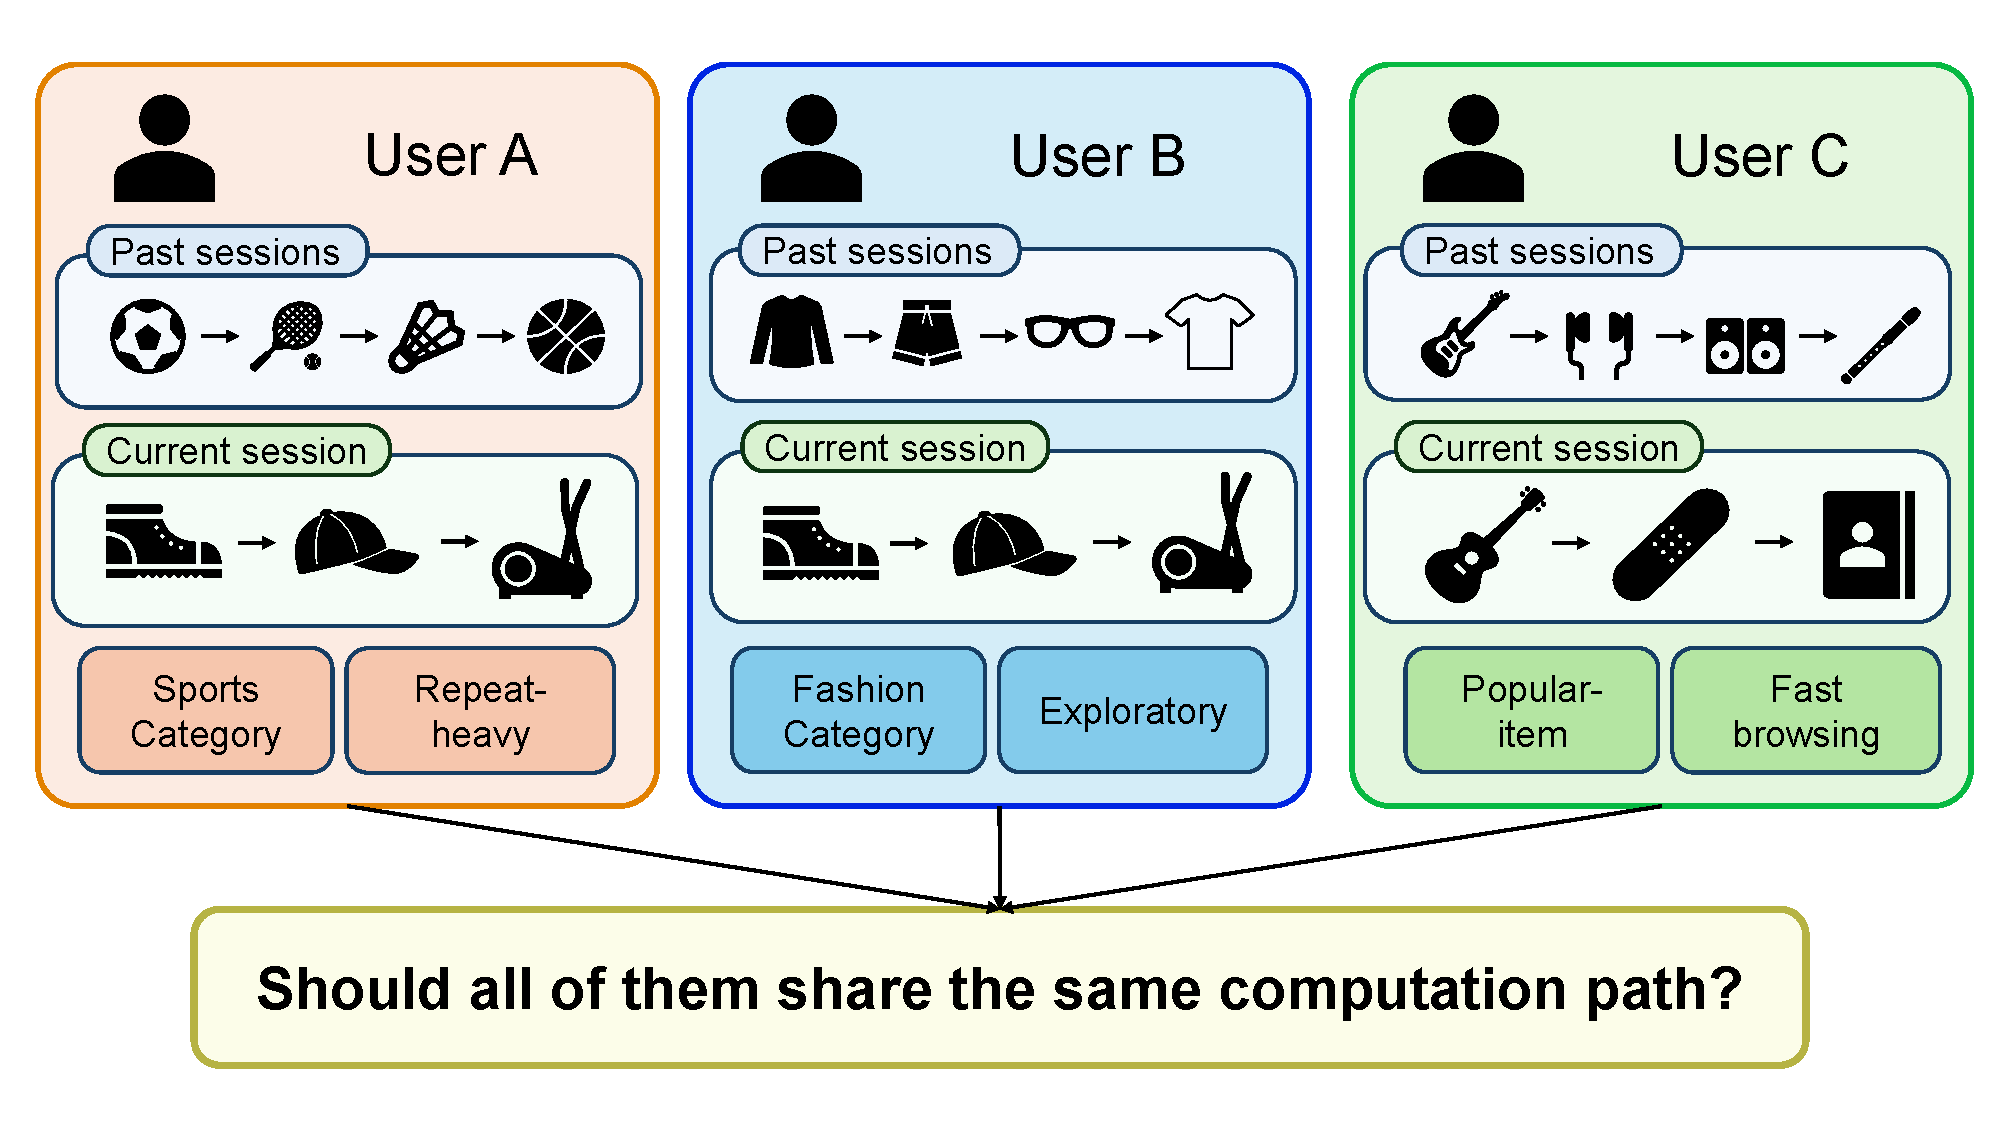
\includegraphics[width=\columnwidth]{figures/figure1_different_user.pdf}
%   \caption{Sessions with different behavioral character still receive the same shared computation in standard sequential recommendation, regardless of pace, repetition, or category focus.}
%   \Description{A problem-motivation figure contrasting different user and session behavior patterns, showing that behaviorally different cases are processed with the same computation path in standard sequential recommendation.}
%   \label{fig:intro-behavioral-features}
% \end{figure}
% A different use of behavioral context is to determine \emph{which computation path} the model applies, rather than only what a shared block encodes. Mixture of Experts (MoE) \cite{jacobs1991adaptive,jordan1994hme} replaces a shared transformation with a set of experts, each activated selectively by a learned router, and Sparse MoE \cite{shazeer2017moe,fedus2022switch} makes this efficient by activating only a small subset at a time. These approaches treat routing as a learned black box: the router reads hidden states that are optimized for next-item prediction, not for reflecting behavioral character. Using behavioral context as the explicit routing input, on a path separate from the representation, has not been addressed.

% The question then is what to use instead. Interaction logs contain behavioral evidence that is directly computable before any model transformation: in short sessions, pace, repetition style, and category focus are often more visible in the raw log than in a hidden state that may not yet reflect cross-session patterns. Routing from these gives the router a signal explicitly about how a session behaves. Keeping the two roles separate has a further consequence: when a route changes, the cause traces back to a specific behavioral cue in the log, not to an opaque shift in hidden-state geometry.

% RouteRec instantiates this design through \emph{behavioral cues} (compact scalar summaries derived directly from interaction logs) computed on a routing control path that does not touch the sequential backbone. Behavioral cues are organized into four cue families: Tempo (pace and interval dynamics), Focus (category concentration and category switching), Memory (repetition and recurrence), and Exposure (popularity level and drift). Cues are extracted at three temporal scopes --- macro (cross-session history), mid (within-session dynamics), and micro (short-term local transitions) --- because each scope surfaces different behavioral evidence. The cue bank therefore acts as a portable routing interface: the same summary template applies at all three scopes without dataset-specific engineering.

% Making this separation work raises three concrete design questions: what cues to construct from ordinary logs, at what temporal scopes routing decisions should be made, and how to structure expert selection so that routes genuinely differ across sessions. Section~\ref{sec:problem} formalizes each.

% The main contributions of this work are:
% \begin{itemize}
%   \item We identify the routing input as a key design choice in sessionized sequential recommendation and argue that behavioral cues, computed from interaction logs on a path separate from the sequential backbone, provide a cleaner routing interface than hidden states.
%   \item We propose RouteRec, which implements this design through three components: Behavioral Cue Construction, Coarse-to-Fine Multi-Stage Routing, and Hierarchical Sparse Expert Allocation.
%   \item Empirically, RouteRec achieves the best overall Avg.~Rank in the main comparison across six datasets under a shared sessionized temporal protocol, with the clearest gains on Foursquare, LastFM, and KuaiRec.
% \end{itemize}

\section{Related Work}
\label{sec:related}

\subsection{Session-based and Sequential Recommendation}
Sequential recommendation predicts the next item from an ordered interaction history \cite{wang2019seqsurvey}. Session-based recommendation is a closely related setting in which those interactions are partitioned into short temporally bounded sessions and prediction is made from the current session context \cite{jannach2022sessions,wang2021sessionsurvey}. Earlier models established the main sequence-modeling backbone families for this problem: FPMC \cite{rendle2010fpmc} factorized personalized Markov transitions, Caser \cite{tang2018caser} and NextItNet \cite{yuan2019nextitnet} applied convolutional sequence modeling, and GRU4Rec \cite{hidasi2016gru4rec} showed that recurrent models can learn strong session dynamics. NARM \cite{li2017narm}, STAMP \cite{liu2018stamp}, and SR-GNN \cite{wu2019srgnn} then emphasized session intent, short-term memory, and transition structure more explicitly.

Transformer-based models such as SASRec \cite{kang2018sasrec} and BERT4Rec \cite{sun2019bert4rec} became strong general backbones for sequential recommendation. More recent work adds stronger inductive biases through contrastive regularization \cite{qiu2022duorec,hou2022core}, frequency-aware modeling \cite{du2023fearec,shin2024bsarec}, and selective state-space backbones \cite{liu2025sigma}. These models differ substantially in how they encode the sequence, yet all apply the same shared transformation to every prefix. For short sessions with visibly different structural character, this leaves open whether the model should adapt only its representation or also which transformation it applies.

\subsection{Behavioral Context and Router Inputs}
\jm{Sessions differ not only in which items are selected, but in how: some are repeat-heavy, others exploratory; some stay focused on one category, others shift rapidly.} Hierarchical and session-aware models such as HRNN \cite{quadrana2017hrnn}, SHAN \cite{ying2018shan}, and more recent hybrid session architectures \cite{bauer2024hybridsession} \jm{model long-term user preference and short-term within-session dynamics separately, allowing the representation to reflect both stable tendencies and recent shifts.} Time-aware self-attention \cite{li2020tisasrec} injects interval structure into the backbone. Feature-aware models such as FDSA \cite{zhang2019fdsa} and DIF-SR \cite{xie2022difsr} incorporate side information to refine the sequence representation. RepeatNet \cite{ren2019repeatnet} and ICSRec \cite{qin2024icsrec} focus on repetition and evolving intent. Multi-interest models such as MIND \cite{li2019mind} and ComiRec \cite{cen2020comirec} represent user behavior through multiple latent interests within a single forward pass.

Across these lines of work, behavioral context enriches what the model represents --- injected into hidden states, attention patterns, or auxiliary branches --- while the transformation applied to each prefix remains shared. What has not been addressed is whether compact scalar summaries of session structure — derived directly from interaction logs — can serve as the explicit input to a router, replacing hidden states in the routing control path.

\subsection{Mixture of Experts in Recommendation}

Mixture of Experts (MoE) \cite{jacobs1991adaptive,jordan1994hme} replaces a shared transformation with a router that selects which expert subset to activate. In recommendation, MMoE \cite{ma2018mmoe} and PLE \cite{tang2020ple} use expert decomposition mainly for multi-task learning, where different tasks benefit from different expert subsets. More recent recommendation models such as FAME \cite{liu2025fame}, M3SRec \cite{bian2023m3srec}, and HM4SR \cite{zhang2025hm4sr} also introduce experts, but routing is typically driven by learned hidden representations or modality-specific states rather than by explicit behavioral cues computed from the interaction log.

Sparse MoE \cite{shazeer2017moe,fedus2022switch} makes this conditional computation efficient by activating only a small subset of experts per input.
Sparse MoE mechanics, including expert choice routing \cite{zhou2022expertchoice} and z-loss stabilization \cite{zoph2022stmoe}, improve how expert activation is executed. None of this work addresses what the router should actually read as its input. In session-based recommendation, this is a meaningful gap: session prefixes are short, and the hidden state at routing time may not yet reflect broader behavioral patterns across past sessions. The behavioral reason for any routing decision therefore stays buried in the hidden-state geometry, regardless of the routing mechanism used. RouteRec addresses this by using behavioral cues --- computed directly from the interaction log --- as the explicit router input, on a control path kept separate from the sequential backbone.

\section{Problem and Design Challenges}
\label{sec:problem}

\subsection{Problem Definition}

For each user, let $\mathcal{S}_u=[s_1,\dots,s_M]$ denote the chronologically ordered sequence of sessions, where each session $s_m=[x_{m,1},\dots,x_{m,L_m}]$ contains items interacted with during one continuous activity window. The task is \emph{next-item prediction}: given the current-session prefix $x_{m,1:t}$ and the user's past sessions $[s_1,\dots,s_{m-1}]$, predict the next item $x_{m,t+1}$.

Beyond item identities, interaction logs commonly record when each interaction occurred and what broad category the item belongs to --- temporal timestamps and coarse grouping labels such as category, genre, or artist. Item-level popularity statistics can also be derived from the training corpus itself. We assume these fields are available, as they are in the majority of standard recommendation benchmarks; the method is designed to work best when they are present and degrades gracefully when some are missing. No user profiles, side-information encoders, or auxiliary supervision are required.

\subsection{Design Challenges}

Using explicit behavioral cues as router inputs raises three design challenges. Each one, if left unresolved, causes cue-driven routing to degenerate into a near-uniform mixture that behaves no differently from a shared feed-forward block.

\paragraph{\textbf{C1. Cue portability versus informativeness.}}
Behavioral cues must be computable from whatever fields are present in a given dataset. In practice this means item identities, timestamps, and sometimes a category label --- a narrow set. The risk is that cues built from such a restricted input are too coarse to produce meaningful routing differences across sessions. The challenge is to extract cues that are expressive enough to distinguish behavioral regimes while remaining portable to settings where richer metadata is unavailable.

\paragraph{\textbf{C2. Temporal scope of behavioral evidence.}}
Different behavioral patterns become visible at different time scales. Cross-session tendencies (repetition patterns, long-term drift) only emerge when looking across multiple past sessions. Within-session focus and pacing build up over the current prefix. Local transition dynamics are only apparent in the last few interactions. A single cue vector aggregated over all time scales at once conflates these distinct signals. The challenge is to match routing decisions to the temporal scope at which each type of evidence is most reliable.

\paragraph{\textbf{C3. Route commitment.}}
Even with cue-driven routing, behavior-dependent computation collapses if routing assigns non-negligible weight to all experts. A repeat-heavy session and a fast-exploratory one then activate nearly the same expert mixture, and the routing step adds nothing. The challenge is to concentrate activation on a small, consistent expert subset --- so that behaviorally different sessions genuinely take different computation paths --- without restricting coverage so severely that some behavioral regimes are left unserved.

\begin{figure*}[!t]
  \centering
  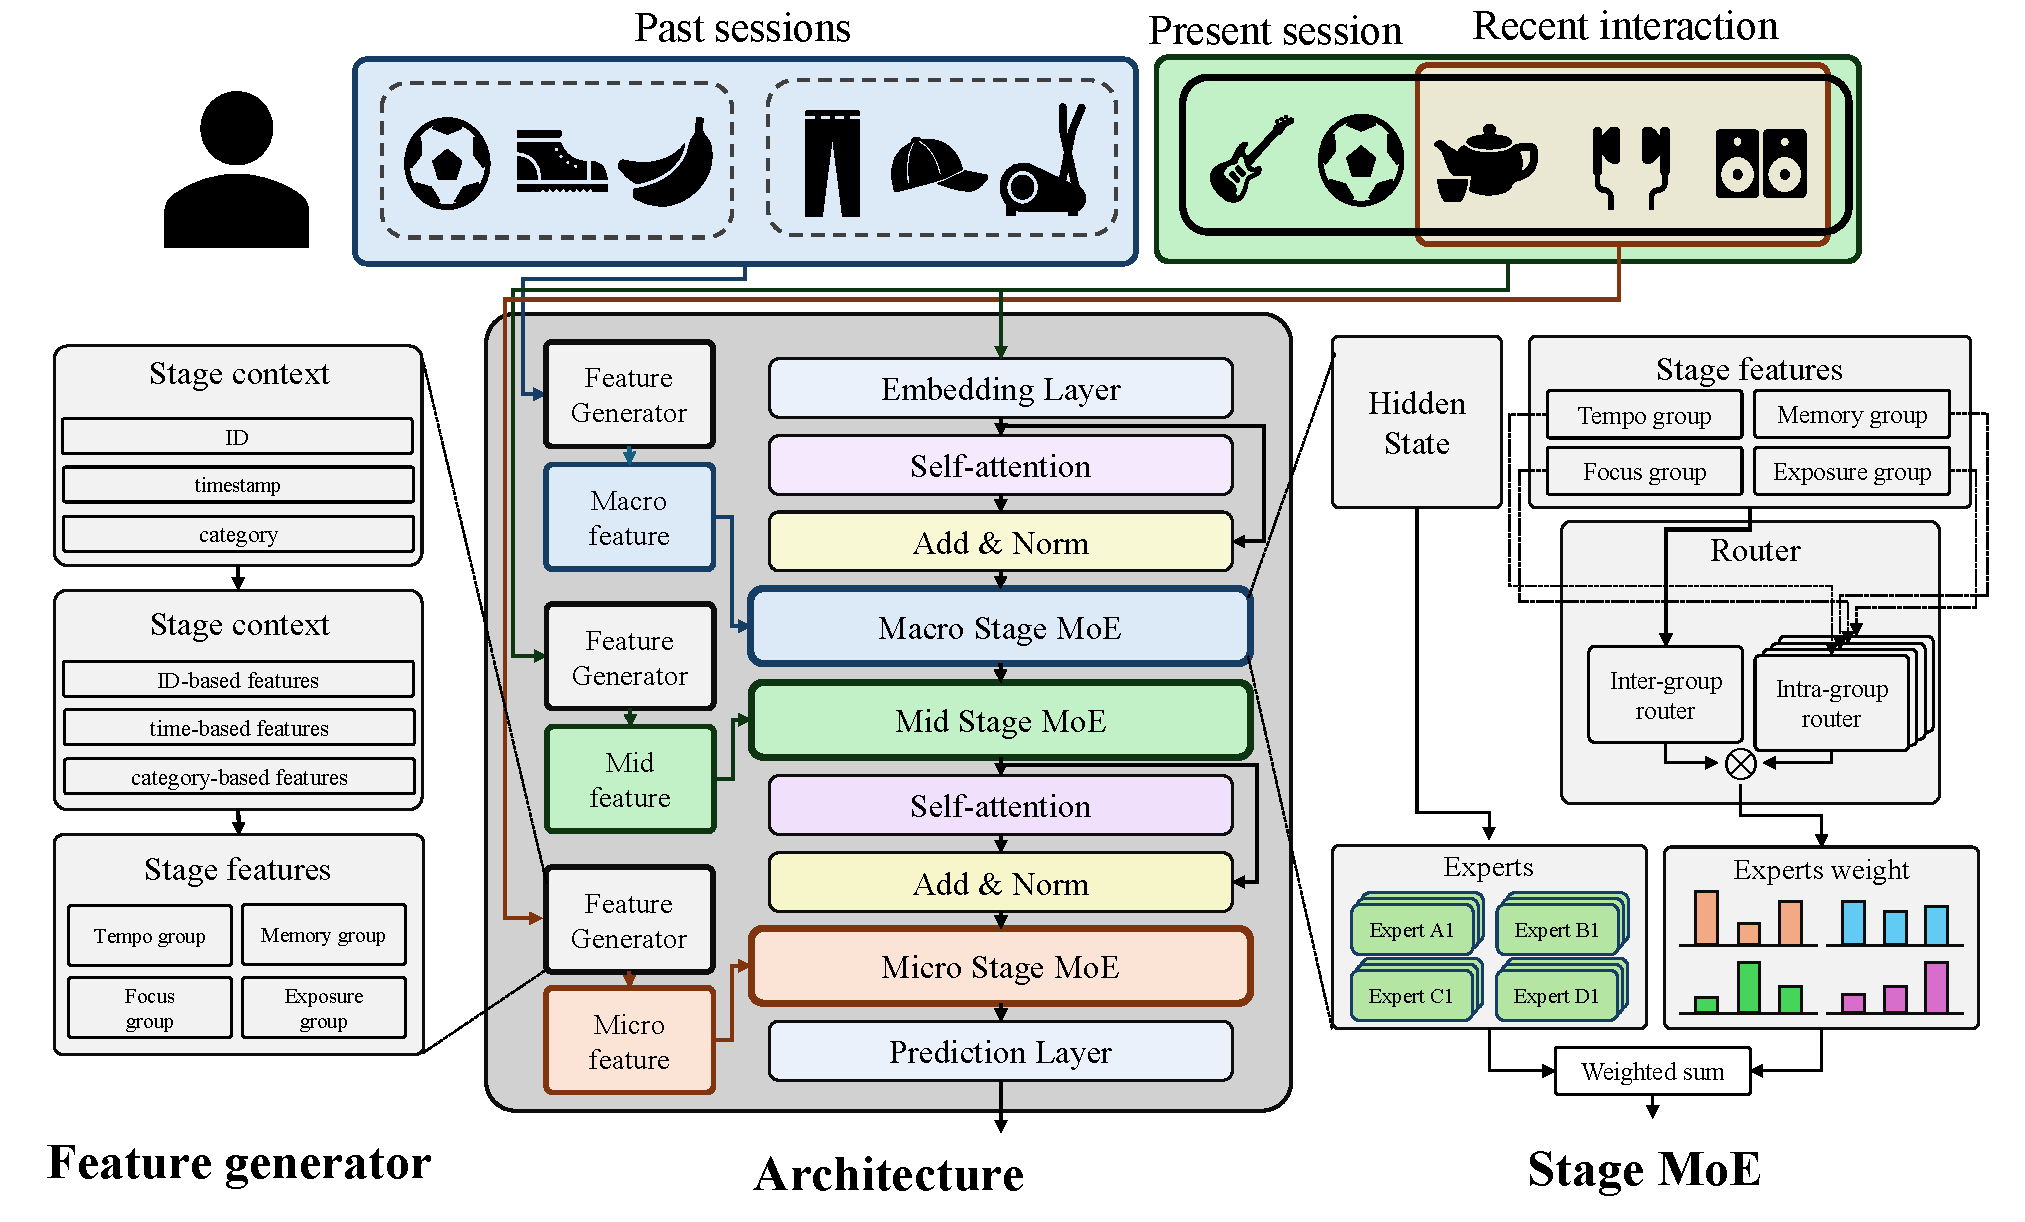
\includegraphics[width=0.95\textwidth]{figures/figure2_overall_arch_simple.pdf}
  \caption{RouteRec framework. \textit{Left --- Cue Extraction}: interaction fields (ID, timestamp, category) are summarized into a cue vector organized by four cue families (Tempo, Focus, Memory, Exposure), computed separately at each temporal scope. \textit{Center --- Architecture}: sequential backbone with macro, mid, and micro routing stages in series. \textit{Right --- Hierarchical Sparse Router}: each stage uses the same two-level router --- a family-level router selects which cue families drive computation, and a within-group router selects specific experts inside each chosen family. Details in Section~\ref{sec:multi-stage-routing} and Appendix~\ref{app:method-details}.}
  \Description{A three-panel architecture figure of RouteRec. Left panel shows cue extraction from interaction fields into a cue vector organized by four cue families. Center panel shows the sequential backbone with macro, mid, and micro routing stages in series. Right panel shows the hierarchical sparse router with a family-level router and within-group router producing a weighted expert mixture.}
  \label{fig:framework}
\end{figure*}

\section{Proposed Method}
\label{sec:method}

RouteRec replaces the shared feed-forward blocks in a SASRec-style backbone with sparse, behavior-guided routing stages. The design is built around two separate paths that operate independently: a \emph{sequential backbone} that encodes the interaction sequence into hidden states for next-item prediction, and a \emph{routing control path} that reads behavioral cues from the interaction log and decides which expert subset processes each input. Hidden states do not drive routing; behavioral cues do not modify the sequence representation.

\subsection{Overview}
\label{sec:routerec-overview}

Figure~\ref{fig:framework} shows the full framework. Three components, each targeting one of the design challenges in Section~\ref{sec:problem}, form the routing control path.

\textbf{Behavioral Cue Construction} (C1) extracts compact scalar summaries from the interaction log --- covering pace, repetition, category focus, and popularity exposure --- organized into four cue families. The same cue structure is applied at three temporal windows, so the method does not require dataset-specific feature engineering.

\textbf{Coarse-to-Fine Multi-Stage Routing} (C2) places one routing stage at each temporal scope --- macro (cross-session), mid (within-session), micro (local) --- interleaved with self-attention blocks. Each stage reads the behavioral cues from its own window, ensuring that routing decisions are made at the time scale where the underlying evidence is most informative.

\textbf{Hierarchical Sparse Expert Allocation} (C3) structures expert selection as a two-level choice: first select which behavioral dimensions (cue families) drive computation, then select specific experts within each chosen family. Activation is restricted to a small subset at both levels, ensuring that behaviorally different sessions take genuinely different computation paths. Alternative configurations for routing stage placement are in Appendix~\ref{app:method-details}.

\subsection{Behavioral Cue Construction}
\label{sec:feature-construction}

The routing control path computes behavioral cues directly from the interaction log, without passing through the sequential backbone. Given a window of interactions $\mathcal{R}$, a shared summary function $\mathcal{A}(\cdot)$ produces a fixed-size \emph{cue vector} $\mathbf{f} = \mathcal{A}(\mathcal{R})$ consisting of scalar statistics computed from the raw log fields.

A key design question is what behavioral dimensions the cue vector should cover. The cues must be (1) computable from commonly available log fields, (2) expressive enough to distinguish sessions with different behavioral character, and (3) consistent across datasets so that no per-dataset feature engineering is needed. We organize the cue vector into four \emph{cue families}, each targeting one observable axis of session behavior:
\begin{itemize}
  \item \textbf{Tempo} --- interaction pace and time-interval dynamics. Captures how fast a session moves: short gaps between interactions indicate an active, rapid-fire session; long gaps suggest deliberate browsing.
  \item \textbf{Focus} --- category concentration and switching patterns. Captures whether a session stays narrowly within one topic area or hops broadly across categories.
  \item \textbf{Memory} --- repetition rate and item recurrence. Captures whether a session revisits previously seen items, a strong signal of exploratory versus habitual behavior.
  \item \textbf{Exposure} --- popularity level and drift across the window. Captures whether the items consumed lean toward mainstream or niche, and whether that preference is shifting.
\end{itemize}
Together, these four families span the structural space that most clearly separates behavioral regimes in session-based recommendation --- how a session moves (Tempo), what it focuses on (Focus), whether it repeats (Memory), and what popularity tier it operates in (Exposure) --- using only fields available in standard interaction logs. Tempo and Memory require only item IDs and timestamps; Exposure uses corpus-level popularity counts; Focus requires a coarse grouping label and falls back to a fixed default when absent, while the other three families continue to drive routing. Representative cue definitions are in Table~\ref{tab:appendix-feature-families}; exact dimensions are in Appendix~\ref{app:method-details}.

The same four-family structure is applied at three temporal windows (macro, mid, micro), described in the next subsection. Because the cue template is fixed across all windows and datasets, no dataset-specific feature engineering is required.

\subsection{Coarse-to-Fine Multi-Stage Routing}
\label{sec:multi-stage-routing}

The central design question here is: \emph{at what temporal scope should routing decisions be made?} Different behavioral patterns become reliable at different scales. A user's tendency to revisit past items is only visible when looking across multiple sessions. Whether the current session is staying focused on one category becomes clear as the prefix grows. The very next item's transition pattern is only apparent in the last few interactions. Collapsing all of these into a single routing decision made at one fixed point in the network would force the router to handle evidence from incompatible time scales simultaneously --- and lose the ability to respond to any one of them cleanly.

RouteRec addresses this by placing a dedicated routing stage at each temporal scope, each reading behavioral cues computed from its own window of history. For session $s_m$ at prediction target $t$, the three windows are:
\begin{align}
\mathcal{R}^{\mathrm{macro}}_t &= [s_{\max(1,m-H)},\dots,s_{m-1}], \\
\mathcal{R}^{\mathrm{mid}}_t   &= [x_{m,1},\dots,x_{m,t-1}], \\
\mathcal{R}^{\mathrm{micro}}_t &= [x_{m,\max(1,t-w)},\dots,x_{m,t-1}],
\end{align}
where $H$ is the number of past sessions and $w$ the local window size. Applying $\mathcal{A}(\cdot)$ to each window gives stage-specific cue vectors $\mathbf{f}^{(\mathrm{macro})}_t$, $\mathbf{f}^{(\mathrm{mid})}_t$, $\mathbf{f}^{(\mathrm{micro})}_t$.

What each stage is designed to capture reflects the nature of its window:
\begin{itemize}
  \item \textbf{Macro} covers the user's recent past sessions. It reflects stable behavioral tendencies --- how broadly the user has ranged across categories, how much they tend to repeat, what popularity tier they typically operate in. These patterns are slow to change and best captured at the cross-session scale.
  \item \textbf{Mid} covers the current session prefix. It reflects how this session is unfolding --- how focused or scattered it has been, how fast it is moving. These properties emerge gradually and are only visible after seeing several interactions within the session.
  \item \textbf{Micro} covers the last few interactions immediately before the target. It reflects the immediate transition context --- the local pattern that most directly precedes the next item.
\end{itemize}

The three stages are interleaved with self-attention blocks in the backbone. Self-attention contextualizes token representations before each routing stage acts on them. This interleaved design ensures routing transforms a properly contextualized hidden state rather than raw embeddings. In the main configuration:
\[
\underbrace{\text{self-attn}}_{\text{contextualize}} \to \text{macro} \to \text{mid} \to \underbrace{\text{self-attn}}_{\text{refresh}} \to \text{micro}.
\]
Macro and mid are both \emph{sequence-level} decisions. Cross-session tendency and within-session dynamics are properties of the whole session, not of individual positions --- a session that has been repeat-heavy is repeat-heavy everywhere, not just at one token. It therefore makes sense to compute one routing decision per sequence (from averaged cue vectors) and apply it uniformly. Micro, by contrast, is \emph{position-level}: local transition patterns differ at each step, so micro computes a separate routing decision per position. A second self-attention block before micro re-contextualizes token representations after macro and mid routing have modified them, ensuring micro routing acts on up-to-date hidden states. Full formulations are in Appendix~\ref{app:method-details}.

Section~\ref{sec:hierarchical-routing} describes how expert selection within each stage enforces route commitment.

\subsection{Hierarchical Sparse Expert Allocation}
\label{sec:hierarchical-routing}

Even with cue-driven routing, the computation path becomes meaningless if routing spreads weight across all experts. A repeat-heavy session and a fast-exploratory one would then activate nearly the same mixture regardless of their cues, and the routing step would add nothing. The key design requirement is \emph{route commitment}: routing must concentrate activation on a small, consistent expert subset so that behaviorally different sessions genuinely take different computation paths.

A secondary requirement is \emph{interpretability of the routing decision}. If expert selection is a flat top-$k$ choice across all $E$ experts, it is hard to understand what behavioral property drove the choice --- one activated expert might relate to repetition, another to pace, another to popularity, with no structural separation between them. A hierarchical structure that first selects \emph{which behavioral dimension} drives computation, then selects \emph{which expert} within that dimension, makes the routing decision directly readable from the cue families.

RouteRec satisfies both requirements through a two-level hierarchical router. The $E$ experts are grouped into $G$ \emph{expert groups} of $C$ experts each ($E = GC$), where each group is aligned with one cue family (Tempo, Focus, Memory, or Exposure). Routing proceeds in two steps: first select which cue families drive computation (family-level), then select specific experts within each chosen family (within-group).

\paragraph{Router formulation.}
The router takes the cue vector $\mathbf{f}^{(s)}_t$ as input and produces two distributions via learned linear projections: a family-level distribution $p^{(s)}_{t,g}$ over expert groups, and a within-group distribution $r^{(s)}_{t,g,c}$ over experts inside each group. Their product $\pi^{(s)}_{t,g,c} = p^{(s)}_{t,g} \cdot r^{(s)}_{t,g,c}$ gives the joint weight for expert $(g,c)$. The factored form is key: it forces the model to first commit to which behavioral dimension matters, then pick the best expert for that dimension --- rather than applying a flat top-$k$ over all experts at once. The same router structure is shared across all three stages; stages differ only in which cue vector they receive.

\paragraph{Sparse selection.}
Route commitment is enforced by hard top-$k$ selection at both levels: only the top-$k_g$ expert groups and the top-$k_e$ experts within each are active, with their weights renormalized. All other experts contribute nothing to the output. Let $\operatorname{TopK}(\mathbf{v},k)$ be the index set of the $k$ largest entries of $\mathbf{v}$; the sparse group weights $\bar{p}^{(s)}_{t,g}$ and within-group weights $\bar{r}^{(s)}_{t,g,c}$ are:
\begin{equation}
\bar{p}^{(s)}_{t,g} = \frac{p^{(s)}_{t,g}\,\mathbf{1}[g\in \operatorname{TopK}(\mathbf{p}^{(s)}_t,k_g)]}{\sum_{g'} p^{(s)}_{t,g'}\,\mathbf{1}[g'\in \operatorname{TopK}(\mathbf{p}^{(s)}_t,k_g)]},
\label{eq:sparse-route}
\end{equation}
\begin{equation}
\bar{r}^{(s)}_{t,g,c} = \frac{r^{(s)}_{t,g,c}\,\mathbf{1}[c\in \operatorname{TopK}(\mathbf{r}^{(s)}_{t,g,:},k_e)]}{\sum_{c'} r^{(s)}_{t,g,c'}\,\mathbf{1}[c'\in \operatorname{TopK}(\mathbf{r}^{(s)}_{t,g,:},k_e)]}.
\label{eq:sparse-within-group}
\end{equation}
The stage output sums only over active experts ($\hat{\pi}^{(s)}_{t,g,c} = \bar{p}^{(s)}_{t,g}\,\bar{r}^{(s)}_{t,g,c}$):
\begin{equation}
\tilde{\mathbf{h}}^{(s)}_t = \sum_{g,c}\hat{\pi}^{(s)}_{t,g,c}\,\mathrm{Expert}^{(s)}_{g,c}(\mathbf{h}^{\mathrm{in},(s)}_t).
\label{eq:sparse-stage-routing}
\end{equation}
Sparsity here is about commitment, not computational efficiency: it ensures that two sessions with different cues cannot end up on the same route just because the soft weights happen to average out the same way. Dense soft mixing --- where every expert contributes a small nonzero weight --- is evaluated as an ablation in Appendix~\ref{app:sparse-design}. Configuration values ($G$, $C$, $k_g$, $k_e$) are in Appendix~\ref{app:method-details}.

\subsection{Training Objective}
\label{sec:training-objective}

RouteRec is trained end-to-end with one prediction loss and two routing regularizers. The routing regularizers are not optional add-ons: without them, cue-driven routing can degenerate in two distinct ways that the prediction loss alone cannot prevent.

\paragraph{Prediction loss.}
The main objective is standard next-item cross-entropy. Let $\mathbf{z}$ be the final logit vector over all items and $y$ the target item:
\[
\mathcal{L}_{\mathrm{CE}} = -\log \frac{\exp(z_y)}{\sum_{j}\exp(z_j)}.
\]
This loss drives the model to rank the correct next item highly, but it provides no direct signal about whether the routing is cue-sensitive or not.

\paragraph{Route consistency.}
The first failure mode: the router ignores behavioral cues and routes all sessions identically, effectively collapsing back to a shared feed-forward block. Route consistency regularization addresses this failure mode by requiring sessions with similar behavioral cues to produce similar routing distributions. For each stage $s$ and sample $i$, let $\bar{\mathbf{f}}^{(s)}_i = \frac{1}{L_i}\sum_t\mathbf{f}^{(s)}_{i,t}$ be the session-level cue average and $\bar{\boldsymbol{\pi}}^{(s)}_i = \frac{1}{L_i}\sum_t\boldsymbol{\pi}^{(s)}_{i,t}$ the corresponding average routing distribution. We pair each sample with its nearest cue neighbor in the mini-batch by $\ell_2$ distance in cue space (pair set $\mathcal{P}_s$) and penalize the divergence between their routing distributions:
\[
\mathcal{L}_{\mathrm{cons}}
=
\frac{1}{|\mathcal{T}|}
\sum_{s \in \mathcal{T}}
\frac{1}{|\mathcal{P}_s|}
\sum_{(i,j)\in \mathcal{P}_s}
\mathrm{JSD}\!\left(\bar{\boldsymbol{\pi}}^{(s)}_i,\,\bar{\boldsymbol{\pi}}^{(s)}_j\right).
\]
This encourages the router to produce routing distributions that reflect the structure of the cue space, not just whatever pattern minimizes the prediction loss.

\paragraph{Routing logit stabilization.}
The second failure mode is subtler: even when the router tries to be cue-sensitive, the pre-softmax logits can grow very large during training. When this happens, the softmax saturates and routing collapses to a near-hard assignment, making small cue differences invisible to the router --- the cue vector stops mattering in practice even though the router nominally reads it. We address this with z-loss \cite{zoph2022stmoe}, which penalizes the scale of the pre-softmax expert logits $a_{i,t,g,c}^{s}$ to keep the routing distribution in a well-behaved range where cue differences can produce meaningfully different outputs:
\[
\mathcal{L}_{z}
=
\frac{1}{|\mathcal{T}|}
\sum_{s \in \mathcal{T}}
\frac{1}{N_s}
\sum_{(i,t)\in\mathcal{V}_s}
\!\left(\log \sum_{g,c}\exp a_{i,t,g,c}^{\,s}\right)^{\!2},
\]
where $\mathcal{V}_s$ is the set of valid positions and $N_s=|\mathcal{V}_s|$. The final objective is:
\[
\mathcal{L} = \mathcal{L}_{\mathrm{CE}} + \lambda_{\mathrm{cons}}\,\mathcal{L}_{\mathrm{cons}} + \lambda_{z}\,\mathcal{L}_{z}.
\]
We do not include a load-balancing term. Classical MoE training often penalizes unequal expert usage to prevent collapse onto a small subset. Here the goal is the opposite: behaviorally distinct sessions should activate different, committed routes rather than distributing traffic evenly. Route consistency and logit stabilization together are sufficient for stable, cue-aligned specialization.

\section{Experiments}
\label{sec:experiments}

\subsection{Experimental Setup}

\paragraph{Datasets and protocol.}
We evaluate on six public datasets: Beauty~\cite{mcauley2015amazon}, Foursquare~\cite{yang2015foursquare}, KuaiRec~\cite{gao2022kuairec}, LastFM~\cite{celma2010music}, ML-1M~\cite{harper2015movielens}, and Retail Rocket~\cite{retailrocket2015dataset}. All datasets are preprocessed under a shared sessionized temporal protocol: interactions are sorted chronologically, grouped into sessions by inactivity threshold, and filtered to remove short sessions and low-support items. The resulting sessions are split chronologically into 70\%/15\%/15\% train/validation/test partitions, and the prediction task is next-item prediction for the last item of each held-out session. KuaiRec and LastFM are large; we use 20\% and 3\% random subsets respectively, and all baselines are evaluated on the same data. Full preprocessing details and dataset statistics are in Appendix~B.

\paragraph{Metrics.}
We report Hit Rate (HR@$k$), Normalized Discounted Cumulative Gain (NDCG@$k$), and Mean Reciprocal Rank (MRR@$k$) at $k \in \{5, 10, 20\}$. All evaluations use the seen-target setting, where the candidate set consists of items observed during training. This is standard practice for ID-based sequential recommendation, which cannot score items outside the training vocabulary~\cite{latifi2021sessionaware}. The primary reported metrics are HR@10, NDCG@10, and MRR@20.

\paragraph{Baselines.}
We compare against nine baselines in three groups.
\textit{Conventional sequential models} --- GRU4Rec~\cite{hidasi2016gru4rec}, SASRec~\cite{kang2018sasrec}, TiSASRec~\cite{li2020tisasrec} --- cover recurrent and self-attention backbones and represent the standard shared-computation baseline.
\textit{Representation-enhanced models} --- DuoRec~\cite{qiu2022duorec}, FEARec~\cite{du2023fearec}, BSARec~\cite{shin2024bsarec} --- improve over the standard backbone through contrastive regularization or frequency-aware encoding, but still apply the same transformation to every session.
\textit{Side-information and MoE models} --- FDSA~\cite{zhang2019fdsa}, DIF-SR~\cite{xie2022difsr}, FAME~\cite{liu2025fame} --- incorporate external item features or expert decomposition; they are the closest comparison to RouteRec in that they go beyond a purely shared backbone.
All methods use the same processed data, the same optimization family, matched early stopping, and the same model-selection rule. Tuning details are in Appendix~B.

\begin{table*}[!t]
  \caption{Test results under the sessionized temporal protocol. Datasets marked with $^\dagger$ are sampled processed subsets (KuaiRec 20\%, LastFM 3\%). For each method, we report the test metrics of the run achieving the highest mean test score over the nine reported metrics. Avg.~Rank is computed over all rows in this table, where lower is better. The RouteRec column is shaded for readability.}
  \label{tab:main-overall}
  \centering
  \small
  \setlength{\tabcolsep}{3.4pt}
  \renewcommand{\arraystretch}{1.05}
  \resizebox{\textwidth}{!}{%
  \begin{tabular}{ll*{9}{c}>{\columncolor{routerecgray}}c}
    \toprule
    Dataset & Metric & SASRec & GRU4Rec & TiSASRec & FEARec & DuoRec & BSARec & FAME & DIF-SR & FDSA & RouteRec \\
    \midrule
    \multirow{3}{*}{Beauty}
      & HR@10   & 0.1324 & 0.0840 & 0.1235 & \tblsecond{0.1404} & 0.1347 & 0.0726 & 0.0497 & 0.1165 & 0.1318 & \tblbest{0.1561} \\
      & NDCG@10 & 0.0800 & 0.0457 & 0.0831 & 0.0797 & 0.0793 & 0.0504 & 0.0303 & 0.0811 & \tblsecond{0.0918} & \tblbest{0.0948} \\
      & MRR@20  & 0.0659 & 0.0361 & 0.0735 & 0.0634 & 0.0662 & 0.0450 & 0.0250 & 0.0716 & \tblbest{0.0822} & \tblsecond{0.0794} \\
    \midrule
    \multirow{3}{*}{Retail Rocket}
      & HR@10   & 0.5321 & 0.5048 & 0.5131 & \tblsecond{0.5487} & 0.5478 & 0.4655 & 0.4612 & 0.4322 & 0.5343 & \tblbest{0.5608} \\
      & NDCG@10 & 0.3907 & 0.3674 & 0.3755 & \tblsecond{0.3998} & 0.3994 & 0.3957 & 0.3943 & 0.3863 & 0.3848 & \tblbest{0.4148} \\
      & MRR@20  & 0.3507 & 0.3290 & 0.3368 & 0.3581 & 0.3576 & \tblbest{0.3745} & \tblsecond{0.3738} & 0.3709 & 0.3427 & 0.3737 \\
    \midrule
    \multirow{3}{*}{Foursquare}
      & HR@10   & 0.3049 & 0.2180 & 0.2976 & 0.3054 & \tblsecond{0.3195} & 0.2383 & 0.2417 & 0.3032 & 0.3042 & \tblbest{0.3215} \\
      & NDCG@10 & 0.1929 & 0.1476 & 0.1926 & 0.1925 & 0.1970 & 0.1609 & 0.1604 & 0.2008 & \tblsecond{0.2014} & \tblbest{0.2042} \\
      & MRR@20  & 0.1624 & 0.1286 & 0.1635 & 0.1613 & 0.1631 & 0.1393 & 0.1378 & \tblsecond{0.1723} & \tblbest{0.1726} & 0.1715 \\
    \midrule
    \multirow{3}{*}{ML-1M}
      & HR@10   & 0.1423 & 0.1456 & 0.1448 & 0.1490 & 0.1555 & 0.1374 & 0.1533 & 0.0669 & \tblbest{0.1606} & \tblsecond{0.1568} \\
      & NDCG@10 & 0.0717 & 0.0778 & 0.0756 & 0.0736 & 0.0810 & 0.0723 & \tblsecond{0.0818} & 0.0331 & \tblbest{0.0833} & 0.0807 \\
      & MRR@20  & 0.0555 & 0.0621 & 0.0600 & 0.0559 & 0.0641 & 0.0570 & \tblsecond{0.0651} & 0.0256 & \tblbest{0.0655} & 0.0631 \\
    \midrule
    \multirow{3}{*}{LastFM$^\dagger$}
      & HR@10   & 0.3775 & 0.3109 & 0.3715 & \tblsecond{0.3876} & 0.3850 & 0.3475 & 0.3359 & 0.3593 & 0.3762 & \tblbest{0.3965} \\
      & NDCG@10 & 0.3097 & 0.2676 & 0.3029 & 0.3187 & 0.3066 & 0.3044 & 0.2972 & 0.3169 & \tblsecond{0.3247} & \tblbest{0.3307} \\
      & MRR@20  & 0.2897 & 0.2558 & 0.2831 & 0.2981 & 0.2833 & 0.2915 & 0.2861 & 0.3051 & \tblsecond{0.3103} & \tblbest{0.3113} \\
    \midrule
    \multirow{3}{*}{KuaiRec$^\dagger$}
      & HR@10   & 0.3284 & 0.3061 & 0.3216 & \tblsecond{0.3513} & 0.3468 & 0.3359 & 0.3307 & 0.2333 & 0.3453 & \tblbest{0.3669} \\
      & NDCG@10 & 0.3177 & 0.2589 & 0.2889 & \tblsecond{0.3286} & 0.3215 & 0.3209 & 0.3188 & 0.2229 & 0.3197 & \tblbest{0.3467} \\
      & MRR@20  & 0.3150 & 0.2462 & 0.2802 & \tblsecond{0.3227} & 0.3153 & 0.3170 & 0.3160 & 0.2201 & 0.3133 & \tblbest{0.3425} \\
    \midrule
    \multicolumn{2}{l}{\textbf{Avg.~Rank$\downarrow$}} & \textbf{6.06} & \textbf{8.67} & \textbf{6.61} & \textbf{4.22} & \textbf{4.17} & \textbf{6.61} & \textbf{6.72} & \textbf{6.72} & \textbf{3.56} & \textbf{1.67} \\
    \bottomrule
  \end{tabular}}
\end{table*}

\subsection{Main Comparison}
\label{sec:overall-performance}

Table~\ref{tab:main-overall} reports seen-target ranking results on all six datasets. We use Avg.~Rank as the primary summary metric, since absolute score scales differ substantially across datasets. RouteRec achieves the best overall Avg.~Rank (1.67 vs.\ 3.56 for FDSA, the next-best baseline).

\begin{table}[t]
  \caption{Per-dataset routing condition and RouteRec gain over the best baseline on HR@10. Session variability and cross-session context availability are proxy indicators described in Appendix~B; gain is positive when RouteRec leads.}
  \label{tab:routing-condition}
  \centering
  \footnotesize
  \setlength{\tabcolsep}{4pt}
  \renewcommand{\arraystretch}{1.07}
  \begin{tabular}{lccc}
    \toprule
    Dataset & Session variability & Context avail. & HR@10 gain \\
    \midrule
    Foursquare   & high   & moderate & \textbf{+XX.X\%} \\
    LastFM       & high   & high     & \textbf{+XX.X\%} \\
    KuaiRec      & high   & moderate & \textbf{+XX.X\%} \\
    Beauty       & moderate & low    & +XX.X\% \\
    Retail Rocket & moderate & low   & +XX.X\% \\
    ML-1M        & low    & high     & +XX.X\% \\
    \bottomrule
  \end{tabular}
\end{table}

Table~\ref{tab:routing-condition} summarizes the routing conditions and observed gains per dataset. The pattern is consistent with the design premise: RouteRec gains most where behavioral variation across sessions is pronounced and cross-session context is available for macro-scope routing. On Beauty and Retail Rocket the margins are smaller, as short and sparse sessions limit the behavioral signal available to the router. On ML-1M, sessions are long and preference-driven; shared computation already captures the dominant behavioral regime, leaving little \emph{routing headroom} --- the degree to which routed computation can improve on a strong shared-path model.

The closest baselines are FDSA, DIF-SR, and FAME, which go beyond a shared backbone through side information or expert decomposition. FDSA and DIF-SR incorporate external features but keep a shared transformation. FAME introduces expert decomposition but routes from hidden states, entangling route choices with the prediction objective. RouteRec's advantage over this group is most pronounced where routing headroom is high, consistent with the claim that explicit behavioral cues provide a cleaner routing signal than hidden states.

\subsection{Cue Portability (C1)}
\label{sec:cue-portability}

Behavioral cues require item IDs, timestamps, and category labels. A practical question is whether the method remains effective when some sources are unavailable. We retrain RouteRec from scratch under three reduced-cue conditions --- removing category cues, removing timestamp cues, or removing both --- and compare against the full model and the best baseline.

\begin{figure}[!t]
  \centering
  
\includegraphics[width=\columnwidth]{figures/fig_q4_portability_legend.pdf}
  \vspace{0.25em}
  \subcaptionbox{KuaiRec}{%
    
\includegraphics[width=0.485\columnwidth]{figures/fig_q4_portability_a.pdf}
  }\hfill
  \subcaptionbox{Foursquare}{%
    
\includegraphics[width=0.485\columnwidth]{figures/fig_q4_portability_b.pdf}
  }
  \caption{Reduced-cue variants on KuaiRec and Foursquare. Each panel compares the full model against no-category, no-timestamp, and sequence-only variants retrained from scratch, with the best baseline shown for reference.}
  \Description{One-column figure with a full-width portability legend above two subfigures for KuaiRec and Foursquare.}
  \label{fig:cue-portability-panels}
\end{figure}

Figure~\ref{fig:cue-portability-panels} shows that reduced-cue variants are generally competitive with the best baseline on HR@10, even when category or timestamp cues are removed. Each source contributes, and the relative benefit differs between datasets. The full model performs best overall, but the gap between partial-cue and full-cue variants is modest, suggesting that behavior-guided routing does not depend on any single metadata source to remain effective.

\subsection{Temporal Scope and Routing Design (C2, C3)}
\label{sec:stage-structure}

RouteRec addresses C2 (Section~\ref{sec:problem}) by distributing routing across three temporal scopes and C3 by enforcing hierarchical sparse expert selection within each stage. We test both design choices with ablations on KuaiRec.

\begin{figure}[!t]
  \centering
  
\includegraphics[width=0.485\columnwidth]{figures/fig_q3_design_justification_a_legend.pdf}\hfill
  
\includegraphics[width=0.485\columnwidth]{figures/fig_q3_design_justification_b_legend.pdf}
  \vspace{0.25em}
  \subcaptionbox{Temporal scopes}{%
    
\includegraphics[width=0.485\columnwidth]{figures/fig_q3_design_justification_a.pdf}
  }\hfill
  \subcaptionbox{Routing organization}{%
    
\includegraphics[width=0.485\columnwidth]{figures/fig_q3_design_justification_b.pdf}
  }
  \caption{Design ablations on KuaiRec. Panel~(a): full three-scope design vs.\ the best-performing reduced variants across scope-removal and parallel weighted-sum configurations. Panel~(b): hierarchical sparse vs.\ flat routing (expert selection across all cues without family structure) and dense activation (all experts active, no top-$k$) under comparable expert budgets.}
  \Description{One-column figure with two half-width legends above two subfigures. Both panels are measured on KuaiRec.}
  \label{fig:stage-structure-panels}
\end{figure}

Panel~(a) compares the three-scope design against the best result from a range of reduced alternatives. These include scope-removal variants (dropping one or two stages entirely) and parallel variants (replacing the serial macro$\to$mid$\to$micro pipeline with a weighted sum of independently computed stage outputs). Removing any scope degrades performance, with the largest drop when the macro scope is absent: cross-session behavioral tendency cannot be recovered from within-session evidence alone. Panel~(b) examines routing organization. Flat routing selects experts directly from the full cue vector without family structure; dense activation removes the top-$k$ constraint and activates all experts simultaneously. Both underperform the hierarchical sparse design under a comparable expert budget, showing that family-level structure and sparse commitment each contribute independently to route quality.

\subsection{Cue Dependence}
\label{sec:cue-efficacy}

The ablations above show that the three-scope structure and hierarchical sparse design are necessary. A separate question is whether the trained router is actually sensitive to the content of the behavioral cue vector, or whether it has learned to ignore cues and route based on other signals.

\begin{figure}[!t]
  \centering
  
\includegraphics[width=\columnwidth]{figures/fig_q4_efficacy_legend.pdf}
  \vspace{0.25em}
  \subcaptionbox{KuaiRec}{%
    
\includegraphics[width=0.485\columnwidth]{figures/fig_q4_portability_c.pdf}
  }\hfill
  \subcaptionbox{Foursquare}{%
    
\includegraphics[width=0.485\columnwidth]{figures/fig_q4_portability_d.pdf}
  }
  \caption{Inference-time cue perturbation on KuaiRec and Foursquare. The trained model is evaluated under intact cues, cross-sample permutation, full zeroing, and intra-sequence permutation. All perturbations corrupt the behavioral identity of the cue vector without changing the backbone.}
  \Description{One-column figure with a full-width cue-efficacy legend above two subfigures for KuaiRec and Foursquare.}
  \label{fig:cue-efficacy-panels}
\end{figure}

We fix the trained model and apply three inference-time perturbations: cross-sample permutation (shuffling cue vectors across the batch), full zeroing, and intra-sequence permutation (shuffling values within each sample). All three corrupt the behavioral identity of the cue without changing the backbone. Figure~\ref{fig:cue-efficacy-panels} shows consistent performance drops across all perturbations on both datasets, confirming that the router has learned to map specific cue content to specific routes. The performance gain depends on the router directing each session to a cue-appropriate computation path, not merely on having routing capacity available.

\subsection{Routing Control}
\label{sec:routing-control}

The preceding studies assume behavioral cues as the routing input. A more fundamental question is whether cue-driven routing outperforms hidden-state-driven routing. Hidden states are optimized for next-item prediction rather than for reflecting behavioral character, and routing from them ties the control path to the very representation it is meant to influence.

\begin{figure}[!t]
  \centering
  
\includegraphics[width=\columnwidth]{figures/fig_q2_routing_control_legend.pdf}
  \vspace{0.25em}
  \subcaptionbox{KuaiRec}{%
    
\includegraphics[width=0.485\columnwidth]{figures/fig_q2_routing_control_a.pdf}
  }\hfill
  \subcaptionbox{Foursquare}{%
    
\includegraphics[width=0.485\columnwidth]{figures/fig_q2_routing_control_b.pdf}
  }
  \caption{Routing-input ablations on KuaiRec and Foursquare. Five variants: shared FFN (no routing), hidden-state-only routing, additive fusion bias, mixed hidden+cue routing, and the final behavior-guided router.}
  \Description{One-column figure with a full-width routing-control legend above two subfigures. The left subfigure reports KuaiRec and the right subfigure reports Foursquare.}
  \label{fig:routing-control-panels}
\end{figure}

Figure~\ref{fig:routing-control-panels} compares five routing-input variants on KuaiRec and Foursquare. Hidden-only routing improves over the shared FFN, and mixing hidden states with behavioral cues adds further gain. The behavior-guided router, which keeps the routing control path fully separate from the sequential backbone, yields the most consistent results across both datasets. Separating the two paths --- rather than enriching the router's input --- is the key factor.

\section{Conclusion}
\label{sec:conclusion}
RouteRec asks whether behavioral cues from ordinary interaction logs can serve as an explicit routing signal for conditional computation in sessionized sequential recommendation, rather than only as inputs for representation enrichment. The answer from the experiments is largely affirmative.

RouteRec achieves the best overall seen-target Avg.~Rank across six datasets, with the clearest gains on datasets where sessions exhibit high behavioral variability and sufficient cross-session history is available. The ablations show that each design component carries its weight: all three temporal scopes are necessary, hierarchical sparse selection outperforms flat and dense alternatives, and the router is demonstrably sensitive to the content of the behavioral cue vector. The gains hold even when only partial metadata is available, though the full cue set performs best.

The broader point is that MoE in session-based recommendation is not just a capacity question. Once conditional computation is available, what drives expert allocation becomes a meaningful design choice. RouteRec's contribution is to make that choice explicit --- using lightweight, interpretable behavioral cues on a control path kept separate from prediction --- and to show that doing so produces consistent gains over strong shared-computation baselines.

\clearpage
\balance
\bibliographystyle{ACM-Reference-Format}
\bibliography{refs}

\clearpage
\appendix

\section{Exact RouteRec Instantiation and Sparse Routing Formulation}
\label{app:method-details}
This appendix records the fixed paper instantiation and the representative cue bank used by RouteRec. Whereas the main text emphasizes the conceptual design axes, this section documents the implementation choices that are relevant for reproducibility and for interpreting the later ablations, with the sparse routing formulation made explicit.

\subsection{Main Paper Configuration}

\begin{table}[H]
  \centering
  \caption{Fixed main configuration used in the paper.}
  \label{tab:appendix-main-setting}
  \footnotesize
  \setlength{\tabcolsep}{4pt}
  \renewcommand{\arraystretch}{1.07}
  \begin{tabularx}{\columnwidth}{@{}L{0.30\columnwidth}>{\raggedright\arraybackslash}X@{}}
    \toprule
    Aspect & Main paper configuration \\
    \midrule
    Backbone layout & self-attn $\to$ macro block $\to$ mid block $\to$ self-attn $\to$ micro block \\
    Stage execution & Serial \\
    Routing granularity & Macro and mid: sequence-wise; micro: position-wise \\
    Router composition & Shared hierarchical sparse router at all three stages \\
    Expert activation & Top-$3$ expert groups out of $4$; top-$2$ experts per selected group \\
    Active experts & $6$ out of $12$ total per routed decision \\
    History windows & $H=5$ sessions (macro); $w=5$ positions (micro) \\
    Core auxiliary terms & Route consistency + z-loss; no load balancing \\
    \bottomrule
  \end{tabularx}
\end{table}

The placement of the two attention layers reflects the intended temporal roles of the stages. The first attention layer contextualizes the raw prefix before any routing is applied. Macro and mid then operate consecutively because both provide slower sequence-level control over the same contextualized sequence state: macro captures broader recent-history tendency, while mid refines within-session evolution. A second attention layer is inserted only before micro so that the final local router receives a refreshed token interaction state immediately before prediction. This layout was the most stable high-performing architecture in our architecture sweep.

This table serves as a reproducibility summary rather than as a search-space description. Architectural choices are fixed across the paper track, whereas capacity and optimization values are selected per dataset from a narrow candidate set and are therefore reported as compact ranges only when no single global value is shared across all reported runs.

\subsection{Implementation Specification and Minimal Execution Notes}

\begin{table}[H]
  \centering
  \caption{Implementation-level settings used in the selected paper track.}
  \label{tab:appendix-implementation-spec}
  \footnotesize
  \setlength{\tabcolsep}{4pt}
  \renewcommand{\arraystretch}{1.07}
  \begin{tabularx}{\columnwidth}{@{}L{0.30\columnwidth}>{\raggedright\arraybackslash}X@{}}
    \toprule
    Item & Reported setting \\
    \midrule
    Cue families & $G=4$ expert groups: Tempo, Focus, Memory, Exposure \\
    Experts per group & $C\in\{2,3,4\}$; total experts $E=4C$ \\
    Main sparse setting & $C=3$, top-$3$ expert groups, top-$2$ experts per selected group \\
    Cue dimensionality & $16$ scalars per stage \\
    Router hidden width & Representative range $48$--$128$ \\
    Routing temperature & Macro $1.0$; mid and micro $1.2$ \\
    Consistency neighbors & $k_{\mathrm{nn}}=1$ nearest non-self sample per stage \\
    Missing-signal handling & Broadcast when available; zero-fill focus cues if grouping field absent \\
    \bottomrule
  \end{tabularx}
\end{table}

\noindent\textbf{Minimal execution notes.}
The implementation uses three simple rules that are easy to miss if one only reads the high-level method description. First, macro and mid cues are computed once per example and then broadcast over the routed positions, whereas micro cues are evaluated at the position level. Second, top-$k$ masking is followed by re-normalization inside the active support rather than by leaving the logits in an unnormalized sparse state. Third, if a dataset does not expose the grouping field needed for focus-family cues, the implementation falls back to the fixed missing-signal policy in Table~\ref{tab:appendix-implementation-spec} rather than silently redefining the cue family per dataset.

\subsection{Representative Behavioral Cue Families}

\begin{table*}[!t]
  \centering
  \caption{Representative cue summaries used by RouteRec in the main configuration. Each stage uses four semantic families with four scalar summaries per family; the table lists representative examples rather than every implementation detail.}
  \label{tab:appendix-feature-families}
  \footnotesize
  \setlength{\tabcolsep}{4pt}
  \renewcommand{\arraystretch}{1.05}
  \begin{tabularx}{\textwidth}{@{}lXXX@{}}
    \toprule
    Family & Macro (recent-session tendency) & Mid (within-session evolution) & Micro (short-horizon pressure) \\
    \midrule
    Tempo & Context-valid ratio, last inter-session gap, mean pace, pace trend & Valid-prefix ratio, mean/std interaction interval, session age & Last gap, short-window mean gap, short-window std, deviation from mid-scale pace \\
    Focus & Theme entropy, dominant-theme mass, theme repeat rate, theme shift rate & Category entropy, category top-1 mass, category switch rate, category uniqueness & Immediate category switch, mismatch to recent category history, suffix entropy, suffix uniqueness \\
    Memory & Repeat intensity, adjacent category overlap, adjacent item overlap, repeat trend & Item uniqueness, repeat rate, novelty rate, longest item run & Reconsumption flag, suffix reconsumption rate, suffix item uniqueness, suffix longest run \\
    Exposure & Mean popularity, popularity spread, popularity entropy, popularity trend & Mean popularity, popularity std, popularity entropy, popularity drift & Last-item popularity, suffix popularity spread, suffix popularity entropy, deviation from mid-scale popularity \\
    \bottomrule
  \end{tabularx}
\end{table*}

This cue bank is intentionally compact. The feature families are hand-designed in the sense that they encode behavioral hypotheses, but the design goal is to keep them as a small set of summaries that can serve as a stable routing interface across datasets. In practice, the macro bank is instantiated from the recent-session window used by the selected paper instantiation, while mid and micro are computed from the current session prefix at different temporal scopes. The main text therefore reports the family structure and representative examples, while this appendix provides the implementation-oriented view.

\section{Dataset, Evaluation, and Full Ranking Results}

All experiments were conducted on machines equipped with NVIDIA RTX 3090 24\,GB GPUs. Each training or evaluation process used a single GPU; multiple GPUs were used only to run independent experiments in parallel, not for multi-GPU training within a single run.
\label{app:data-details}
This appendix summarizes the six datasets and makes the evaluation protocol explicit, since recent work has shown that session construction and split strategy can materially affect offline recommender results~\cite{ji2023leakage,gusak2025timesplit}. The original releases are cited here for completeness~\cite{mcauley2015amazon,yang2015foursquare,gao2022kuairec,celma2010music,harper2015movielens,retailrocket2015dataset}. The dataset descriptions emphasize domain differences and signal availability because the routing branch depends on which behavioral evidence is exposed in each corpus.

\subsection{Datasets and Protocol}

\begin{table}[H]
  \caption{Datasets used in the experiments. Datasets marked with $^\dagger$ are sampled processed subsets.}
  \label{tab:appendix-datasets}
  \centering
  \footnotesize
  \setlength{\tabcolsep}{3.0pt}
  \begin{tabular*}{\columnwidth}{@{\extracolsep{\fill}}llrrrc@{}}
    \toprule
    Dataset & Domain & Interactions & Sessions & Items & Avg. len. \\
    \midrule
    Beauty & E-com. & 33,488 & 4,243 & 3,625 & 7.9 \\
    Foursquare & POI & 145,238 & 25,369 & 30,588 & 5.7 \\
    KuaiRec$^\dagger$ & Video & 287,411 & 24,458 & 6,477 & 11.8 \\
    LastFM$^\dagger$ & Music & 470,408 & 25,089 & 52,510 & 18.8 \\
    ML-1M & Movie & 575,281 & 14,539 & 3,533 & 39.6 \\
    Retail Rocket & Browse & 821,243 & 153,092 & 90,211 & 5.4 \\
    \bottomrule
  \end{tabular*}
\end{table}

Table~\ref{tab:appendix-datasets} reports the statistics of the final processed datasets used in the experiments rather than the raw corpus sizes. In particular, KuaiRec corresponds to the 20\% processed subset used in our runs, and LastFM corresponds to the 3\% processed subset.

For reproducibility, the protocol is summarized as follows.
\begin{enumerate}
  \item Sort all interactions chronologically within each dataset.
  \item Reconstruct sessions with a dataset-specific inactivity threshold.
  \item Iteratively prune sessions with length below $5$ and items with support below $3$ until the constraints are simultaneously satisfied.
  \item Sort the resulting sessions by session start time.
  \item Assign the earliest 70\% of sessions to train and treat the latest 30\% as a held-out tail.
  \item Build validation and test from the held-out tail under chronology-preserving cleanup.
  \item Report seen-target metrics as the primary view and keep unseen-target behavior as supplementary accounting.
\end{enumerate}

Beauty and Retail Rocket stress sparse e-commerce revisit behavior, Foursquare and KuaiRec emphasize stronger short-horizon intent changes, and LastFM and ML-1M provide longer preference-driven histories. This spread makes it possible to examine whether behavior-guided routing is primarily beneficial in highly dynamic settings or remains competitive when preference structure is more stable.

Signal availability also differs in a way that matters for routing. Beauty exposes item, time, and product-category cues after low-rating removal. Foursquare includes item, timestamp, and venue-category structure with bursty check-in dynamics. KuaiRec offers item, time, and coarse content-side metadata in short-video sessions with strong short-term intent shifts. LastFM provides repeated listening histories with artist-side signals, while ML-1M contributes longer preference-driven sequences with genre information. Retail Rocket is the sparsest side-information setting, relying mainly on anonymous event streams with item and time signals.

We position our setup as a sessionized sequential evaluation protocol assembled from established components, not as the canonical raw-sequence protocol for sequential recommendation~\cite{jannach2022sessions,quadrana2017hrnn,latifi2021sessionaware}. Sessions are reconstructed post hoc with inactivity heuristics, which is standard practice when logs do not provide explicit session boundaries. The thresholds are adapted to the logging regime of each corpus: Foursquare, KuaiRec, LastFM, ML-1M, and Retail Rocket use a 30-minute inactivity threshold, consistent with dense-log session-aware practice~\cite{quadrana2017hrnn,lacic2020jobsessions}, whereas Beauty uses a 14-day threshold because review timestamps are substantially more diffuse. More generally, this threshold choice reflects the observation that sparse and item-poor domains often require longer or more domain-specific notions of a session than dense clickstream data~\cite{borgbruun2022insurance}. After sessionization, we repeatedly remove sessions shorter than $5$ and items with fewer than $3$ interactions until no further pruning is required. This iterative filtering follows the same general rationale as common session-based benchmark preprocessing, where short sessions and very low-support items are filtered to stabilize next-item supervision and evaluation~\cite{li2017narm,wu2019srgnn}.

Session splits are constructed at the session level after sorting by session start time. The earliest 70\% of sessions are assigned to training, and the remaining 30\% are treated as a held-out tail. This tail is first divided into validation and test using stratification over three factors: whether the target item already appears in the prefix, the target item's popularity bucket with respect to the training split, and the session-length bucket. For the final evaluation files, we then merge the held-out sessions, restore chronological order, and re-split them contiguously into equal validation and test halves. This chronology-preserving design is meant to reduce leakage and keep the offline protocol aligned with temporal deployment order~\cite{ji2023leakage,gusak2025timesplit}.

For the primary evaluation view, we report seen-target metrics only. Concretely, in the held-out files, non-target rows whose items are unseen in training are removed, and unseen targets are retained only for supplementary accounting rather than the main comparison. This matches long-standing session-based and session-aware evaluation practice for ID-based recommendation models, which cannot rank targets outside the training vocabulary and therefore typically separate unseen-target behavior from the primary benchmark table~\cite{latifi2021sessionaware}. We report HR, NDCG, and MRR at $k\in\{5,10,20\}$ for all methods.

For the result tables, each method is represented by the run with the highest mean seen-target test score over the nine reported metrics under the same selection rule used throughout the paper.

All methods use the same processed train/validation/test partitions. RouteRec's additional macro, mid, and micro cues are deterministic summaries derived from those same observed histories, so the comparison should be read as evaluating different ways of exploiting the shared sessionized interaction context rather than different access to held-out information.

\subsection{Model Selection and Tuning Protocol}

Because this benchmark is built from a sessionized temporal protocol rather than a canonical raw-sequence leaderboard, the model-selection procedure is stated explicitly. Prior benchmark studies have shown that both baseline quality and model ranking can change materially once methods are re-evaluated under a common framework and retuned under a shared protocol~\cite{latifi2021sessionaware,latifi2022seqstudy}. Accordingly, the comparison does not rely on paper defaults alone.

Our reporting protocol follows three simple rules. First, every model is tuned within a predefined bounded search space that is fixed before the final comparison: learning rate is sampled log-uniformly within a declared dataset-specific interval, while the remaining hyperparameters are drawn from small predeclared candidate sets. Second, these bounded spaces cover a shared core of optimization hyperparameters together with a small number of model-specific controls, so that the search is broad enough to avoid trivial under-tuning but still budgeted tightly enough to remain comparable across methods. Third, the final reported result for every model is the test performance of the configuration that maximizes the mean validation score over the nine reported metrics. When adaptive search is used for computational efficiency, it is restricted to the same predeclared bounds and candidate sets and should therefore be read as an efficient implementation of a controlled bounded search rather than as open-ended retuning~\cite{galuzzi2020bayesopt}.

The final paper track therefore uses bounded search spaces rather than unconstrained retuning. In the paper-facing comparison, baselines and RouteRec are aligned to the same shared optimization pool, and model families differ only through a small number of architecture-specific additions. For RouteRec, the selected three-stage routing layout remains fixed, but depth, hidden dropout, and routing-side controls are still tuned within bounded candidate sets. To keep the appendix concise but still reproducible, Table~\ref{tab:appendix-final-grid} separates the shared optimization pool from the baseline-family and RouteRec-specific additions, and lists the dataset-specific learning-rate intervals explicitly.

\begin{table*}[!t]
  \centering
  \caption{Bounded candidate grids used in the final paper track.}
  \label{tab:appendix-final-grid}
  \footnotesize

  \begin{minipage}[t]{0.54\textwidth}
    \textbf{(a) Shared Optimization Pool}

    \vspace{0.25em}
    \scriptsize
    \setlength{\tabcolsep}{4pt}
    \renewcommand{\arraystretch}{1.03}
    \begin{tabularx}{\linewidth}{@{}lX@{}}
      \toprule
      Parameter & Candidate sets \\
      \midrule
      Learning rate & Dataset-specific log-uniform interval; see panel (d) \\
      Weight decay & $\{5\times10^{-7},10^{-6},10^{-5},5\times10^{-5},10^{-4},1.5\times10^{-4}\}$ \\
      Max history length & $\{10,20,30\}$ or $\{10,20,30,50\}$ \\
      Width / embedding & $\{64,96,112,128,160\}$ or $\{96,112,128,160,192\}$ \\
      Inner width & $\{128,192,224,256,320\}$ or $\{192,224,256,320,384\}$ \\
      Layers / heads & Layers $\{1,2,3,4\}$; heads $\{1,2,4,8\}$ if applicable \\
      Dropout & Hidden / ratio: $\{0.10,0.12,0.13,0.15,0.18\}$\newline
      Recurrent: $\{0.10,0.15,0.20,0.25,0.30\}$\newline
      Attention: $\{0.06,0.08,0.10,0.12,0.15\}$ or $\{0.08,0.10,0.12,0.15,0.20\}$ \\
      \bottomrule
    \end{tabularx}
  \end{minipage}\hfill
  \begin{minipage}[t]{0.42\textwidth}
    \textbf{(b) Baseline-Family Additions}

    \vspace{0.25em}
    \scriptsize
    \setlength{\tabcolsep}{4pt}
    \renewcommand{\arraystretch}{1.03}
    \begin{tabularx}{\linewidth}{@{}lX@{}}
      \toprule
      Model(s) & Additional candidate sets \\
      \midrule
      TiSASRec & Time span $\{64,128,256,384,512\}$ \\
      GRU4Rec & Recurrent dropout $\{0.10,0.15,0.20,0.25,0.30\}$ \\
      DuoRec / FEARec & $\tau\{0.16,0.18,0.20,0.22,0.24\}$\newline
      Contrastive weight $\{0.02,0.03,0.04,0.05,0.06\}$\newline
      Semantic weight $\{0,0.04,0.05,0.08,0.10\}$ or $\{0.04,0.05,0.08,0.10,0.12\}$ \\
      BSARec & $\alpha\{0.35,0.50,0.55,0.70\}$\newline
      $c\{2,3,5,7\}$ \\
      DIF-SR / FDSA & Attribute width $\{96,128,160,192\}$\newline
      $\lambda_{\mathrm{attr}}$ $\{0.08,0.09,0.10,0.12,0.14\}$ or $\{0.09,0.10,0.12,0.14,0.15\}$ \\
      DIF-SR & Fusion $\{\mathrm{gate},\mathrm{sum},\mathrm{concat}\}$ \\
      FAME & Expert count $\{2,3,4,5,6\}$ \\
      \bottomrule
    \end{tabularx}
  \end{minipage}

  \vspace{0.75em}

  \begin{minipage}[t]{0.50\textwidth}
    \textbf{(c) RouteRec-Specific Additions}

    \vspace{0.25em}
    \scriptsize
    \setlength{\tabcolsep}{4pt}
    \renewcommand{\arraystretch}{1.03}
    \begin{tabularx}{\linewidth}{@{}lX@{}}
      \toprule
      Parameter & Candidate sets \\
      \midrule
      Backbone depth / dropout & Depth: $\{1,2,3\}$\newline
      Dropout: $\{0.10,0.12,0.14,0.15,0.16,0.17\}$\newline
      $\phantom{\text{Dropout: }}\{0.18,0.19,0.20,0.22,0.24\}$ \\
      Weight decay & $\{3.125,5,6,10,15,20,50\}\times10^{-7}$ \\
      Routing capacity & Expert scale $\{2,3,4\}$ or $\{2,3,4,5\}$ for KuaiRec\newline
      router width $\{32,64,96,128\}$ \\
      Routing dropout & Feature $\{0,0.03,0.05,0.10\}$\newline
      attention $\{0.05,0.06,0.08,0.10,0.12\}$ \\
      Regularization & $\lambda_{\mathrm{cons}}\{0,2.5,5,8,12\}\times10^{-4}$\newline
      $\lambda_z\{0,5,10,20\}\times10^{-5}$ \\
      Cue bank & Cue bank size $\{10,12,16,24\}$\newline
      router inner width per cue family (small preset) \\
      \bottomrule
    \end{tabularx}
  \end{minipage}\hfill
  \begin{minipage}[t]{0.42\textwidth}
    \textbf{(d) Dataset-Specific Learning-Rate Intervals}

    \vspace{0.25em}
    \scriptsize
    \setlength{\tabcolsep}{4pt}
    \renewcommand{\arraystretch}{1.03}
    \begin{tabularx}{\linewidth}{@{}lX@{}}
      \toprule
      Dataset & Unified log-uniform LR interval \\
      \midrule
      Beauty & 1.5e-4 $\sim$ 2e-3 \\
      Foursquare & 1.5e-4 $\sim$ 2.2e-3 \\
      KuaiRec & 3e-4 $\sim$ 5e-3 \\
      LastFM & 8e-5 $\sim$ 1.2e-3 \\
      ML-1M & 1.5e-4 $\sim$ 2.2e-3 \\
      Retail Rocket & 1.5e-4 $\sim$ 2.2e-3 \\
      \bottomrule
    \end{tabularx}
  \end{minipage}
\end{table*}

\subsection{Full Ranking Results}
Table~\ref{tab:appendix-full-seen} restores the full cutoff grid summarized more compactly in Table~\ref{tab:main-overall}. This presentation preserves the same selection rule as the main text while exposing the complete $k\in\{5,10,20\}$ breakdown.

The appendix table confirms that the same qualitative ordering persists across cutoffs: RouteRec is strongest overall, SASRec and TiSASRec remain robust reference points, and the relatively weaker BSARec and DIF-SR results are consistent with the sessionized short-prefix regime discussed in Section~\ref{sec:overall-performance} rather than with a change in selection or evaluation policy.

\begin{table*}[!t]
  \caption{Full seen-target experimental results across all cutoffs. Datasets marked with $^\dagger$ are sampled processed subsets. For each method, we report the seen-target test metrics of the run achieving the highest mean seen-target test score over the nine reported metrics. Avg.~Rank is computed over all rows in this table, where lower is better. The RouteRec column is shaded for readability.}
  \label{tab:appendix-full-seen}
  \centering
  \scriptsize
  \setlength{\tabcolsep}{2.6pt}
  \renewcommand{\arraystretch}{0.96}
  \resizebox{0.985\textwidth}{!}{%
  \begin{tabular}{ll*{9}{c}>{\columncolor{routerecgray}}c}
    \toprule
    Dataset & Metric & SASRec & GRU4Rec & TiSASRec & FEARec & DuoRec & BSARec & FAME & DIF-SR & FDSA & RouteRec \\
    \midrule
    \multirow{9}{*}{Beauty}
      & HR@5    & 0.1038 & 0.0573 & 0.0918 & 0.1003 & 0.0993 & 0.0630 & 0.0372 & 0.0993 & \tblsecond{0.1041} & \tblbest{0.1087} \\
      & HR@10   & 0.1324 & 0.0840 & 0.1235 & \tblsecond{0.1404} & 0.1347 & 0.0726 & 0.0497 & 0.1165 & 0.1318 & \tblbest{0.1561} \\
      & HR@20   & 0.1637 & 0.1146 & 0.1630 & 0.1757 & \tblsecond{0.1958} & 0.0955 & 0.0592 & 0.1385 & 0.1681 & \tblbest{0.2009} \\
      & NDCG@5  & 0.0707 & 0.0372 & 0.0729 & 0.0669 & 0.0678 & 0.0474 & 0.0263 & 0.0756 & \tblbest{0.0830} & \tblsecond{0.0798} \\
      & NDCG@10 & 0.0800 & 0.0457 & 0.0831 & 0.0797 & 0.0793 & 0.0504 & 0.0303 & 0.0811 & \tblsecond{0.0918} & \tblbest{0.0948} \\
      & NDCG@20 & 0.0879 & 0.0533 & 0.0931 & 0.0889 & 0.0948 & 0.0563 & 0.0327 & 0.0867 & \tblsecond{0.1011} & \tblbest{0.1062} \\
      & MRR@5   & 0.0598 & 0.0307 & 0.0666 & 0.0556 & 0.0571 & 0.0422 & 0.0228 & 0.0677 & \tblbest{0.0761} & \tblsecond{0.0701} \\
      & MRR@10  & 0.0637 & 0.0341 & 0.0707 & 0.0608 & 0.0619 & 0.0434 & 0.0244 & 0.0700 & \tblbest{0.0796} & \tblsecond{0.0762} \\
      & MRR@20  & 0.0659 & 0.0361 & 0.0735 & 0.0634 & 0.0662 & 0.0450 & 0.0250 & 0.0716 & \tblbest{0.0822} & \tblsecond{0.0794} \\
    \midrule
    \multirow{9}{*}{Retail Rocket}
      & HR@5    & 0.4610 & 0.4312 & 0.4433 & \tblsecond{0.4730} & 0.4711 & 0.4411 & 0.4398 & 0.4262 & 0.4579 & \tblbest{0.4862} \\
      & HR@10   & 0.5321 & 0.5048 & 0.5131 & \tblsecond{0.5487} & 0.5478 & 0.4655 & 0.4612 & 0.4322 & 0.5343 & \tblbest{0.5608} \\
      & HR@20   & 0.5988 & 0.5719 & 0.5810 & \tblsecond{0.6234} & 0.6194 & 0.4887 & 0.4812 & 0.4365 & 0.6053 & \tblbest{0.6315} \\
      & NDCG@5  & 0.3676 & 0.3436 & 0.3528 & 0.3752 & 0.3745 & \tblsecond{0.3877} & 0.3874 & 0.3844 & 0.3600 & \tblbest{0.3907} \\
      & NDCG@10 & 0.3907 & 0.3674 & 0.3755 & \tblsecond{0.3998} & 0.3994 & 0.3957 & 0.3943 & 0.3863 & 0.3848 & \tblbest{0.4148} \\
      & NDCG@20 & 0.4076 & 0.3844 & 0.3926 & \tblsecond{0.4187} & 0.4175 & 0.4015 & 0.3994 & 0.3874 & 0.4028 & \tblbest{0.4327} \\
      & MRR@5   & 0.3365 & 0.3145 & 0.3227 & 0.3427 & 0.3423 & \tblsecond{0.3696} & 0.3695 & \tblbest{0.3698} & 0.3274 & 0.3588 \\
      & MRR@10  & 0.3461 & 0.3243 & 0.3321 & 0.3529 & 0.3526 & \tblbest{0.3729} & \tblsecond{0.3724} & 0.3706 & 0.3377 & 0.3688 \\
      & MRR@20  & 0.3507 & 0.3290 & 0.3368 & 0.3581 & 0.3576 & \tblbest{0.3745} & \tblsecond{0.3738} & 0.3709 & 0.3427 & 0.3737 \\
    \midrule
    \multirow{9}{*}{Foursquare}
      & HR@5    & 0.2350 & 0.1741 & 0.2388 & 0.2403 & 0.2438 & 0.1995 & 0.1954 & 0.2458 & \tblsecond{0.2514} & \tblbest{0.2559} \\
      & HR@10   & 0.3049 & 0.2180 & 0.2976 & 0.3054 & \tblsecond{0.3195} & 0.2383 & 0.2417 & 0.3032 & 0.3042 & \tblbest{0.3215} \\
      & HR@20   & 0.3635 & 0.2593 & 0.3501 & 0.3620 & \tblsecond{0.3760} & 0.2773 & 0.2800 & 0.3536 & 0.3524 & \tblbest{0.3776} \\
      & NDCG@5  & 0.1703 & 0.1334 & 0.1735 & 0.1714 & 0.1726 & 0.1483 & 0.1455 & 0.1821 & \tblbest{0.1843} & \tblsecond{0.1829} \\
      & NDCG@10 & 0.1929 & 0.1476 & 0.1926 & 0.1925 & 0.1970 & 0.1609 & 0.1604 & 0.2008 & \tblsecond{0.2014} & \tblbest{0.2042} \\
      & NDCG@20 & 0.2078 & 0.1580 & 0.2059 & 0.2068 & 0.2114 & 0.1708 & 0.1701 & 0.2135 & \tblsecond{0.2136} & \tblbest{0.2184} \\
      & MRR@5   & 0.1489 & 0.1199 & 0.1519 & 0.1486 & 0.1491 & 0.1313 & 0.1289 & \tblsecond{0.1611} & \tblbest{0.1621} & 0.1588 \\
      & MRR@10  & 0.1583 & 0.1258 & 0.1599 & 0.1574 & 0.1591 & 0.1366 & 0.1351 & \tblsecond{0.1688} & \tblbest{0.1692} & 0.1676 \\
      & MRR@20  & 0.1624 & 0.1286 & 0.1635 & 0.1613 & 0.1631 & 0.1393 & 0.1378 & \tblsecond{0.1723} & \tblbest{0.1726} & 0.1715 \\
    \midrule
    \multirow{9}{*}{ML-1M}
      & HR@5    & 0.0858 & 0.0984 & 0.0906 & 0.0906 & 0.0977 & 0.0892 & 0.0968 & 0.0384 & \tblbest{0.1022} & \tblsecond{0.1005} \\
      & HR@10   & 0.1423 & 0.1456 & 0.1448 & 0.1490 & 0.1555 & 0.1374 & 0.1533 & 0.0669 & \tblbest{0.1606} & \tblsecond{0.1568} \\
      & HR@20   & 0.2157 & 0.2181 & 0.2220 & 0.2234 & \tblsecond{0.2402} & 0.2018 & 0.2243 & 0.1052 & \tblbest{0.2426} & 0.2353 \\
      & NDCG@5  & 0.0536 & 0.0626 & 0.0582 & 0.0549 & 0.0624 & 0.0568 & \tblsecond{0.0637} & 0.0240 & \tblbest{0.0645} & 0.0627 \\
      & NDCG@10 & 0.0717 & 0.0778 & 0.0756 & 0.0736 & 0.0810 & 0.0723 & \tblsecond{0.0818} & 0.0331 & \tblbest{0.0833} & 0.0807 \\
      & NDCG@20 & 0.0902 & 0.0960 & 0.0950 & 0.0923 & \tblsecond{0.1022} & 0.0884 & 0.0996 & 0.0427 & \tblbest{0.1038} & 0.1004 \\
      & MRR@5   & 0.0431 & 0.0510 & 0.0476 & 0.0432 & 0.0508 & 0.0463 & \tblbest{0.0529} & 0.0192 & \tblsecond{0.0522} & 0.0504 \\
      & MRR@10  & 0.0505 & 0.0572 & 0.0548 & 0.0508 & 0.0584 & 0.0527 & \tblbest{0.0603} & 0.0230 & \tblsecond{0.0600} & 0.0577 \\
      & MRR@20  & 0.0555 & 0.0621 & 0.0600 & 0.0559 & 0.0641 & 0.0570 & \tblsecond{0.0651} & 0.0256 & \tblbest{0.0655} & 0.0631 \\
    \midrule
    \multirow{9}{*}{LastFM$^\dagger$}
      & HR@5    & 0.3471 & 0.2836 & 0.3405 & \tblsecond{0.3630} & 0.3521 & 0.3312 & 0.3173 & 0.3389 & 0.3494 & \tblbest{0.3693} \\
      & HR@10   & 0.3775 & 0.3109 & 0.3715 & \tblsecond{0.3876} & 0.3850 & 0.3475 & 0.3359 & 0.3593 & 0.3762 & \tblbest{0.3965} \\
      & HR@20   & 0.3999 & 0.3338 & 0.3997 & \tblsecond{0.4103} & 0.4101 & 0.3615 & 0.3554 & 0.3825 & 0.4020 & \tblbest{0.4194} \\
      & NDCG@5  & 0.2999 & 0.2588 & 0.2929 & 0.3108 & 0.2959 & 0.2992 & 0.2911 & 0.3103 & \tblsecond{0.3161} & \tblbest{0.3218} \\
      & NDCG@10 & 0.3097 & 0.2676 & 0.3029 & 0.3187 & 0.3066 & 0.3044 & 0.2972 & 0.3169 & \tblsecond{0.3247} & \tblbest{0.3307} \\
      & NDCG@20 & 0.3154 & 0.2735 & 0.3101 & 0.3245 & 0.3129 & 0.3080 & 0.3020 & 0.3228 & \tblsecond{0.3313} & \tblbest{0.3365} \\
      & MRR@5   & 0.2841 & 0.2506 & 0.2770 & 0.2933 & 0.2771 & 0.2884 & 0.2822 & 0.3008 & \tblsecond{0.3050} & \tblbest{0.3059} \\
      & MRR@10  & 0.2881 & 0.2542 & 0.2812 & 0.2965 & 0.2815 & 0.2906 & 0.2847 & 0.3035 & \tblsecond{0.3085} & \tblbest{0.3096} \\
      & MRR@20  & 0.2897 & 0.2558 & 0.2831 & 0.2981 & 0.2833 & 0.2915 & 0.2861 & 0.3051 & \tblsecond{0.3103} & \tblbest{0.3113} \\
    \midrule
    \multirow{9}{*}{KuaiRec$^\dagger$}
      & HR@5    & 0.3195 & 0.2770 & 0.3004 & \tblsecond{0.3397} & 0.3270 & 0.3281 & 0.3255 & 0.2275 & 0.3270 & \tblbest{0.3494} \\
      & HR@10   & 0.3284 & 0.3061 & 0.3216 & \tblsecond{0.3513} & 0.3468 & 0.3359 & 0.3307 & 0.2333 & 0.3453 & \tblbest{0.3669} \\
      & HR@20   & 0.3379 & 0.3367 & 0.3429 & \tblsecond{0.3688} & 0.3677 & 0.3464 & 0.3430 & 0.2411 & 0.3654 & \tblbest{0.3949} \\
      & NDCG@5  & 0.3148 & 0.2493 & 0.2820 & \tblsecond{0.3249} & 0.3152 & 0.3184 & 0.3172 & 0.2210 & 0.3140 & \tblbest{0.3410} \\
      & NDCG@10 & 0.3177 & 0.2589 & 0.2889 & \tblsecond{0.3286} & 0.3215 & 0.3209 & 0.3188 & 0.2229 & 0.3197 & \tblbest{0.3467} \\
      & NDCG@20 & 0.3200 & 0.2666 & 0.2942 & \tblsecond{0.3330} & 0.3269 & 0.3236 & 0.3220 & 0.2248 & 0.3248 & \tblbest{0.3538} \\
      & MRR@5   & 0.3133 & 0.2400 & 0.2759 & \tblsecond{0.3200} & 0.3112 & 0.3152 & 0.3144 & 0.2188 & 0.3097 & \tblbest{0.3382} \\
      & MRR@10  & 0.3144 & 0.2441 & 0.2788 & \tblsecond{0.3215} & 0.3138 & 0.3162 & 0.3151 & 0.2196 & 0.3120 & \tblbest{0.3406} \\
      & MRR@20  & 0.3150 & 0.2462 & 0.2802 & \tblsecond{0.3227} & 0.3153 & 0.3170 & 0.3160 & 0.2201 & 0.3133 & \tblbest{0.3425} \\
    \midrule
    \multicolumn{2}{l}{\textbf{Avg.~Rank$\downarrow$}} & \textbf{6.07} & \textbf{8.63} & \textbf{6.56} & \textbf{4.41} & \textbf{4.41} & \textbf{6.52} & \textbf{6.72} & \textbf{6.55} & \textbf{3.40} & \textbf{1.74} \\
    \bottomrule
  \end{tabular}}
\end{table*}

This table makes it possible to verify whether the observed trends persist beyond the compact main-text summary under the same selection rule.

\FloatBarrier

\section{Where RouteRec Helps Most: Special Bins}
\label{app:special-bins}
This section examines coarse difficulty-oriented bins such as session length, target frequency, and optional user history, with the goal of showing where the average RouteRec gain is concentrated. The reported analyses distribute gains across session-length, item-frequency, and optional user-history regimes rather than treating the average result as a black box.

\begin{table}[H]
  \centering
  \caption{Special-bin definitions and sample counts used in the appendix gain analysis.}
  \label{tab:appendix-special-bins}
  \scriptsize
  \setlength{\tabcolsep}{4pt}
  \begin{tabularx}{\columnwidth}{@{}l>{\raggedright\arraybackslash}Xc@{}}
    \toprule
    Bin family & Definition rule & Visualization \\
    \midrule
    Session length & Short / medium / long session buckets from the observed prefix length & Figure~\ref{fig:appendix-special-bins}(a) \\
    Target frequency & Rare / mid / frequent target buckets under the train split & Figure~\ref{fig:appendix-special-bins}(b) \\
    User history & Optional low-history / medium-history / heavy-history grouping & Supporting figure \\
    \bottomrule
  \end{tabularx}
\end{table}

\begin{figure*}[!tbp]
  \centering
  
\includegraphics[width=0.92\textwidth]{figures/appendix/a04_special_bins.pdf}
  \caption{Special-bin analysis reporting where the average RouteRec gain is concentrated across session-length and target-frequency regimes. These bins are coarse difficulty- and exposure-oriented partitions rather than semantically defined behavioral regimes.}
  \Description{Figure showing RouteRec gain across session-length and target-frequency bins.}
  \label{fig:appendix-special-bins}
\end{figure*}

RouteRec produces its clearest seen-target margin in behaviorally heterogeneous or otherwise difficult regimes, consistent with the pattern reported in the main comparison (Section~\ref{sec:overall-performance}).

\section{Extended Framework and Structural Ablations}
\label{app:stage-layout}
This section extends the design-justification study in Section~\ref{sec:stage-structure} by examining broader temporal-layout and cue-organization variants. Figure~\ref{fig:appendix-stage-layout} collects cue-family organization controls and temporal-layout variants that are too detailed for the main text. The goal is to show that the selected architecture is a stable design choice rather than an arbitrary one.

\begin{figure*}[!tbp]
  \centering
  \begin{minipage}[t]{0.48\textwidth}
    \centering
    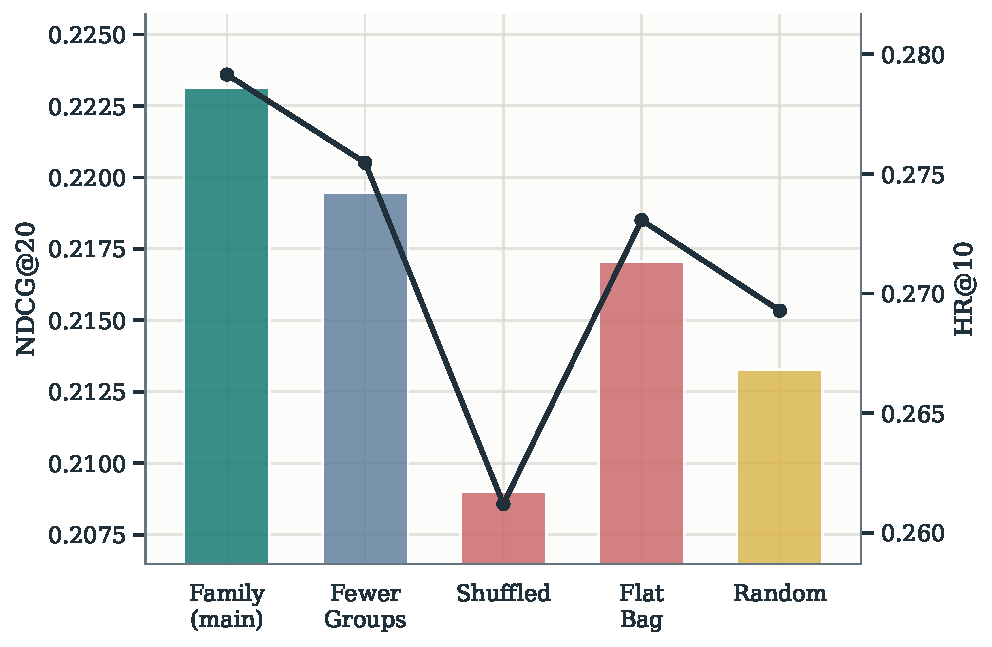
\includegraphics[width=\linewidth]{figures/appendix/a02_structural_cue_org.pdf}
    \vspace{0.1em}
    {\footnotesize (a) Cue-family and expert-group organization variants}
  \end{minipage}\hfill
  \begin{minipage}[t]{0.48\textwidth}
    \centering
    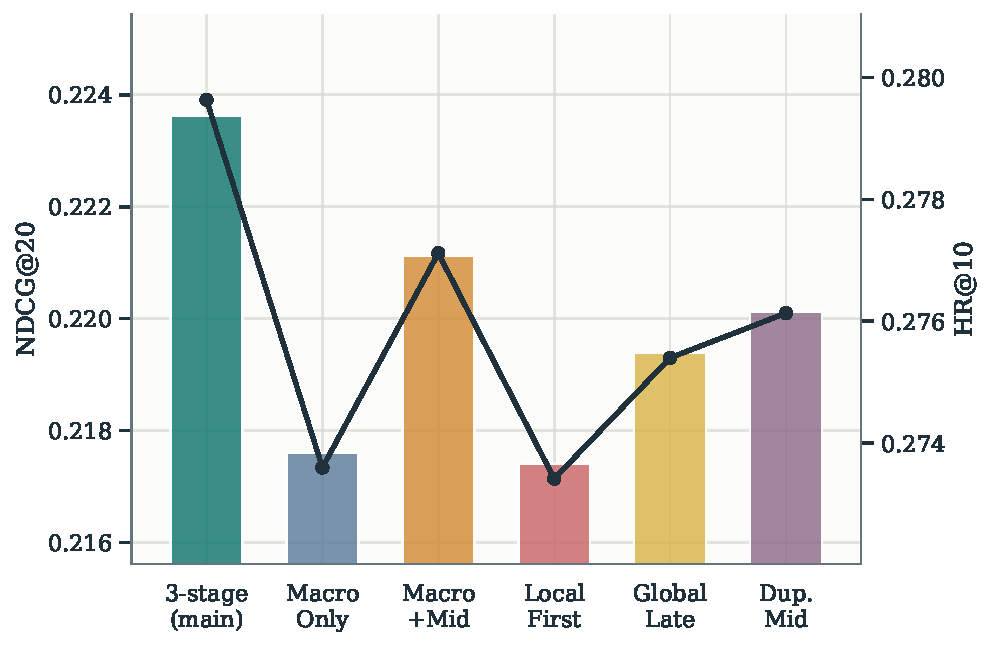
\includegraphics[width=\linewidth]{figures/appendix/a02_structural_temporal.pdf}
    \vspace{0.1em}
    {\footnotesize (b) Stage-semantics and temporal-layout variants}
  \end{minipage}
  \caption{Extended structural ablations. (a) Cue-family and expert-group organization variants. (b) Stage-semantics, temporal-role controls, and layout variants.}
  \Description{Two-panel figure for extended structural ablations: cue-family and expert-group organization variants, and temporal layout variants.}
  \label{fig:appendix-stage-layout}
\end{figure*}

Panel (a) tests whether organizing experts into cue-family-aligned groups matters beyond a flat scalar bag. Panel (b) checks whether the macro, mid, and micro roles correspond to meaningfully distinct temporal views rather than just repeated copies of the same router, and whether the selected stage ordering remains the most stable high-performing layout among the temporal controls.

\section{Sparse Routing Design Variants}
\label{app:sparse-design}
Table~\ref{tab:appendix-sparse-design} tests whether the selected sparse hierarchy is an arbitrary engineering choice or a meaningful part of the RouteRec design. This section directly supports the design-justification study in Section~\ref{sec:stage-structure} by contrasting dense (soft) mixing, flat sparse controls, and hierarchical top-$k$ variants under comparable activation budgets.

\begin{table}[H]
  \centering
  \caption{Sparse routing design variants, ranging from a dense reference to progressively sparser hierarchical configurations under comparable total expert pools.}
  \label{tab:appendix-sparse-design}
  \footnotesize
  \setlength{\tabcolsep}{4pt}
  \begin{tabularx}{\columnwidth}{@{}>{\raggedright\arraybackslash}Xcc>{\raggedright\arraybackslash}X@{}}
    \toprule
    Variant & MRR@20 & Active experts & Observation \\
    \midrule
    Dense full mixture & 0.336 & 12 & Reference control \\
    Flat sparse top-$6$ & 0.335 & 6 & Same active count without hierarchy \\
    Top-$2$ families, top-$1$ex & 0.332 & 2 & Extremely sparse reference \\
    Top-$2$ families, top-$2$ex & 0.335 & 4 & Strong family commitment, tight capacity \\
    Top-$3$ families, top-$2$ex & \textbf{0.339} & 6 & \textbf{Selected main setting} \\
    Top-$4$ families, top-$2$ex & 0.337 & 8 & Weaker family commitment \\
    Top-$3$ families, top-$3$ex & 0.338 & 9 & Larger active-compute budget reference \\
    \bottomrule
  \end{tabularx}
\end{table}

The table separates three related questions: whether sparsity itself helps, whether hierarchy matters beyond a flat top-$k$ mask, and whether the selected main setting provides a reasonable balance between route commitment and active capacity.

\section{Objective and Regularization Variants}
\label{app:objective}
This section isolates whether the observed routing behavior depends primarily on the selected auxiliary objective or remains stable across objective variants. Table~\ref{tab:appendix-objective} reports ranking quality together with routing-stability indicators for each objective configuration.

\begin{table}[H]
  \centering
  \caption{Objective and regularization variants.}
  \label{tab:appendix-objective}
  \footnotesize
  \setlength{\tabcolsep}{4pt}
  \begin{tabularx}{\columnwidth}{@{}>{\raggedright\arraybackslash}XYYY@{}}
    \toprule
    Variant & MRR@20 & Neighbor JSD $\downarrow$ & Route-entropy var.\ $\downarrow$ \\
    \midrule
    No auxiliary loss & 0.333 & 0.148 & 0.094 \\
    KNN consistency only & 0.336 & 0.127 & 0.091 \\
    z-loss only & 0.337 & 0.136 & 0.083 \\
    Balance loss only & 0.334 & 0.141 & 0.090 \\
    Consistency + z-loss & 0.338 & 0.124 & 0.080 \\
    Full objective & \textbf{0.339} & \textbf{0.121} & \textbf{0.079} \\
    \bottomrule
  \end{tabularx}
\end{table}

The two central comparisons are whether the selected objective improves ranking under sparse routing, and whether removing specific auxiliary terms materially changes route sharpness and consistency.

\section{Full Cost and Efficiency Summary}
\label{app:efficiency}
Table~\ref{tab:appendix-efficiency} provides a compact cost summary for the claim that the routing branch is lightweight. Rather than turning the appendix into a systems study, this section reports the rough parameter and runtime overhead for representative baselines together with RouteRec's active-parameter view under sparse routing.

\begin{table}[H]
  \centering
  \caption{Model cost and efficiency summary for all compared methods.}
  \label{tab:appendix-efficiency}
  \scriptsize
  \setlength{\tabcolsep}{3pt}
  \renewcommand{\arraystretch}{1.05}
  \begin{tabularx}{\columnwidth}{@{}L{0.19\columnwidth}ccccL{0.32\columnwidth}@{}}
    \toprule
    Model & Params & Active params & Train $\times$ & Infer $\times$ & Note \\
    \midrule
    GRU4Rec & 1.4 & 1.4 & $0.83\times$ & $0.88\times$ & \makecell[l]{Dense recurrent reference} \\
    SASRec & 1.8 & 1.8 & $1.00\times$ & $1.00\times$ & \makecell[l]{Normalization anchor} \\
    TiSASRec & 2.1 & 2.1 & $1.31\times$ & $1.22\times$ & \makecell[l]{Time-aware Transformer} \\
    DuoRec & 2.0 & 2.0 & $1.28\times$ & $1.15\times$ & \makecell[l]{Contrastive sequential} \\
    FEARec & 2.0 & 2.0 & $1.35\times$ & $1.24\times$ & \makecell[l]{Frequency-aware} \\
    BSARec & 1.9 & 1.9 & $1.18\times$ & $1.10\times$ & \makecell[l]{Structural sequential} \\
    FAME & 2.8 & 2.8 & $1.62\times$ & $1.48\times$ & \makecell[l]{Expert-based baseline} \\
    DIF-SR & 2.4 & 2.4 & $1.42\times$ & $1.32\times$ & \makecell[l]{Feature-aware sequential} \\
    FDSA & 2.3 & 2.3 & $1.38\times$ & $1.28\times$ & \makecell[l]{Feature-side attention} \\
    RouteRec & 3.2 & 1.6 & $1.42\times$ & $1.18\times$ & \makecell[l]{Active params: routed subset only} \\
    \bottomrule
  \end{tabularx}
\end{table}

A compact cost comparison is sufficient here to anchor the selective-activation claim and to show that the observed gains are not being attributed solely to an unchecked increase in compute. The timing numbers in this table are measured on a single NVIDIA RTX 3090 24\,GB GPU under the same batch-size and evaluation conditions; the ratios serve as a practical reference point rather than as a deployment-grade systems benchmark.

\section{Extended Routing Diagnostics}
\label{app:diagnostics}
This section summarizes the final model's routing structure through aggregate diagnostics. Figure~\ref{fig:appendix-diagnostics} collects expert-group usage, route sharpness, and stage-wise consistency so they can be read together.

\begin{figure}[H]
  \centering
  \begin{minipage}[t]{0.48\linewidth}
    \centering
    
\includegraphics[width=\linewidth]{figures/appendix/a03_routing_heatmaps.pdf}
    \vspace{0.1em}
    {\footnotesize (a) Stage-wise family and expert usage heatmaps}
  \end{minipage}\hfill
  \begin{minipage}[t]{0.48\linewidth}
    \centering
    
\includegraphics[width=\linewidth]{figures/appendix/a03_routing_diagnostics_lines.pdf}
    \vspace{0.1em}
    {\footnotesize (b) Route entropy and effective-expert-count summary}
  \end{minipage}
  \caption{Routing diagnostics. (a) Cue-family and expert usage heatmaps by stage. (b) Route entropy and effective expert count across variants.}
  \Description{Two-panel figure showing routing diagnostics: usage heatmaps and route entropy summaries.}
  \label{fig:appendix-diagnostics}
\end{figure}

These diagnostics are organized from coarse structure to semantic interpretation. Panel (a) shows how cue-family selection and expert usage are distributed by stage, while Panel (b) summarizes route sharpness and effective expert usage across the main sparse-routing variants.

\section{Extended Behavioral Slice Results}
\label{app:behavior-slices}
Unlike Appendix~\ref{app:special-bins}, which analyzes coarse difficulty-oriented bins, this section examines semantically defined behavioral regimes: repeat-heavy, fast exploratory, narrow-focus, and preference-stable slices. Each slice is defined by a simple observable statistic of the interaction history, not by optimized supervision targets.

\begin{table}[H]
  \centering
  \caption{Diagnostic slice definitions used in the behavior-regime analysis.}
  \label{tab:appendix-slice-definitions}
  \scriptsize
  \setlength{\tabcolsep}{4pt}
  \begin{tabularx}{\columnwidth}{@{}lX@{}}
    \toprule
    Slice & Definition rule \\
    \midrule
    Repeat-heavy & Prefix repeat ratio above a fixed percentile threshold \\
    Fast-tempo & Mean inter-event gap below a fixed percentile threshold \\
    Narrow-focus & Category or item-transition entropy below a fixed percentile threshold \\
    Exploration-heavy & Novel-item or low-repeat ratio above a fixed percentile threshold \\
    \bottomrule
  \end{tabularx}
\end{table}

These slices are used only for post hoc diagnosis. They are computed from simple observable statistics of the interaction history, not from optimized supervision targets, and not from labels learned jointly with the model.

\begin{figure}[H]
  \centering
  \begin{minipage}[t]{0.58\linewidth}
    \centering
    
\includegraphics[width=\linewidth]{figures/appendix/a04_behavior_slices.pdf}
    \vspace{0.1em}
    {\footnotesize (a) Slice-wise MRR@20 across behavioral regimes}
  \end{minipage}\hfill
  \begin{minipage}[t]{0.38\linewidth}
    \centering
    
\includegraphics[width=\linewidth]{figures/appendix/a04_slice_relative_gain.pdf}
    \vspace{0.1em}
    {\footnotesize (b) Relative RouteRec gain by slice}
  \end{minipage}
  \caption{Extended behavior-regime analysis. (a) Slice-wise ranking quality across behavioral regimes. (b) Relative RouteRec gain over SASRec by behavioral slice.}
  \Description{Two-panel figure for slice-wise MRR@20 and relative RouteRec gain across behavioral regimes.}
  \label{fig:appendix-behavior-slices}
\end{figure}

Together, the two panels expose dataset-level heterogeneity that would be too detailed for the main paper while making the slice construction explicit enough to avoid circular interpretation.

\FloatBarrier

\section{Optional Transfer Results}
\label{app:transfer}
This section reports optional transfer-style results examining whether RouteRec's portable routing interface can be reused across domains with different behavioral and temporal characteristics. The source-target matrix and low-resource curves provide the pairwise and data-efficiency views omitted from the main text.

\begin{figure}[H]
  \centering
  
\includegraphics[width=0.92\columnwidth]{figures/appendix/a06_transfer.pdf}
  \caption{Transfer analysis. Low-resource MRR@20 curves across data fractions comparing full fine-tune, finetuned router, anchor transfer, frozen router, and no-transfer baselines.}
  \Description{Figure showing low-resource transfer curves and transfer-strategy comparisons.}
  \label{fig:appendix-transfer-panels}
\end{figure}

Figure~\ref{fig:appendix-transfer-panels} shows how the routing interface transfers across data-efficiency regimes. Full fine-tuning and finetuned-router transfer consistently outperform the no-transfer baseline, while the frozen-router setting remains a lightweight alternative at higher data fractions.

\end{document}
